\documentclass{UoNMCHA}

% Packages to include
\usepackage[authoryear]{natbib}
\usepackage{array,booktabs} % For nice tables
\usepackage{amsmath,amsfonts,amssymb,mathrsfs,bm} % For nice 
\usepackage{color}
\usepackage{enumerate}
\usepackage{listings}
\usepackage{subfig}
\usepackage{hyperref}
\usepackage[normalem]{ulem}
\usepackage[parfill]{parskip}   % For replacing paragraph indenting with a newline instead

\usepackage{csvsimple} % For tables from CSV
\usepackage{float} % Used for forcing diagrams to the [H] action


\usepackage[shortlabels]{enumitem} % Custom lists

\usepackage{stringstrings}      % Sentence Case
\usepackage[explicit]{titlesec} % Sentence Case




% Wikipedia-style "citation needed" macro source: https://gist.github.com/martinarroyo/b9e0a963ad27169a6eee
\newcommand{\citationneeded}{\textsuperscript{\color{blue} [citation needed]}}
% New macro to make defining labels easier.
\newcommand{\flagforreview}{\textsuperscript{\color{red} [FLAGGED FOR REVIEW]}}
\newcommand{\inlineQuote}[1]{``#1''}
\newcommand{\fancyquote}[1]{\begin{quotation}\inlineQuote{#1}\end{quotation}}
\newcommand{\fref}[1] {Figure \ref{#1}}
\newcommand{\sref}[1] {Section \ref{#1}}
\newcommand{\tref}[1] {Table \ref{#1}}
\newcommand{\aref}[1] {Appendix \ref{#1}}
\newcommand{\fFigure}[3]{
	\begin{figure}[h]
        \begin{center}  
            \includegraphics[width=#3\linewidth]{Figures/#1}  
            \caption{#2}
            \label{#1}
        \end{center}
	\end{figure}
}

\newcommand{\NewSection}[1]{
    \clearpage 
    \section{#1}
}

% \newcommand\SentenceCase[1]{%
%   \caselower[e]{#1}%
%   \capitalize[q]{\thestring}%
% }
% \titleformat{\section}
%   {\normalfont\Large\bfseries}{\thesection}{1em}{\SentenceCase{#1}\thestring}

% \newcommand{\SentenceCaseSubSection}[1]{\subsection{\SentenceCase{#1}}}
% \newcommand{\SentenceCaseSubParagraph}[1]{\subparagraph{}{\SentenceCase{#1}}}

 

%\LoadClass[twoside,a4paper,11pt]{scrartcl}

% Make all math bigger
%\setmathfont{XITS Math}[10pt,version=xits]

%\defaultscriptratio=0.7

% Number equations per section
\numberwithin{equation}{section}

\hypersetup{
%    bookmarks=true,         % show bookmarks bar?
%    unicode=false,          % non-Latin characters in AcrobatÕs bookmarks
%    pdftoolbar=true,        % show AcrobatÕs toolbar?
%    pdfmenubar=true,        % show AcrobatÕs menu?
%    pdffitwindow=false,     % window fit to page when opened
%    pdfstartview={FitH},    % fits the width of the page to the window
    pdftitle={Chris Caelli | FYP Part B Report},    % title
    pdfauthor={Chris Caelli},     % author
    pdfsubject={FYP PART B},   % subject of the document
%    pdfcreator={Creator},   % creator of the document
%    pdfproducer={Producer}, % producer of the document
%    pdfkeywords={keyword1} {key2} {key3}, % list of keywords
%    pdfnewwindow=true,      % links in new window
    colorlinks=true,       % false: boxed links; true: colored links
    linkcolor=blue,          % color of internal links
    citecolor=blue,        % color of links to bibliography
%    filecolor=magenta,      % color of file links
    urlcolor=blue           % color of external links
}

\definecolor{MATLABKeyword}{rgb}{0,0,1}
\definecolor{MATLABComment}{rgb}{0.1328125,0.54296875,0.1328125}
\definecolor{MATLABString}{rgb}{0.625,0.125,0.9375}

\lstset{language=Matlab,
    basicstyle=\small\ttfamily,
    keywordstyle=\color{MATLABKeyword},
    %identifierstyle=,
    commentstyle=\color{MATLABComment},
    stringstyle=\color{MATLABString},
    numberstyle=\tiny,
    %numbers=left,
    basewidth=0.5em}




\firstpage{1}    % Set page number for first page
\UoNMCHAreportNo{MECH4841 Part B} %Report number
\UoNMCHAyear{2019}   % Year
\shorttitle{FYP Report - CCAELLI} %For odd pages
%%%%%%%%%%%%%%%%%%%%%%%%%%%%%%%%%%%%%%%%%%%%%%%%%%%%
\begin{document}
\title{The effect of supplementary data on Acoustic Event Classification through Machine Learning \\ \ \\
{\small Final Year Project Report - MECH4841 Part B  \\JUNE 2019}}
\author[UoNMCHA]{Christopher Caelli}
\address[UoNMCHA]{
Student of Mechatronics Engineering,\\
The University of Newcastle, Callaghan, NSW 2308, AUSTRALIA \\
% Student Number: 3206246 \\
E-mail: \href{mailto:Christopher.Caelli@uon.edu.au}{\textsf{Christopher.Caelli@uon.edu.au}}}
%%%%%%%%%%%%%%%%%%%%%%%%%%%%%%%%%%%
\maketitle
\onecolumn

\vspace{-5mm}
\section*{Mandatory Dot Point Summary}
\vspace{-3mm}

flagforreview \flagforreview \\
citationneeded \citationneeded \\
Tense: Past, Future etc. Search "was", "is" "ed" etc.
Check contraction. it's, don't etc.
check for our, we, I, they're, your, you, etc.
check for st-ray - inca-se the-y block sh-t
check ref and replace with fref, tref, aref etc.
fix header to og %School of Engineering, Discipline of Mechanical Engineering and Mechatronics
check \\refs\{\} for whether the fullstop is before or after
As per the FYP Handbook: \\
I did:
\begin{itemize}
    \item I learnt and prototyped two machine learning solutions that takes audio and physical data (GPS, accelerometer, gyroscope) to compare whether the supplementary data could improve the classification of an acoustic event, as measured by the F1 score.
    \item I learnt and prototyped a pipeline to record data, process it, classify it, and output it.
    \item I used my mechatronics subject matter learnings to best apply machine learning to this problem. This includes Mechatronics Design (trade off and evaluations from MCHA3000), sound pre-processing, preprocessing Inertial Measuring Unit data, and how Audio waveforms can be treated as energy, and statistics from MECH2450/MCHA3900. \flagforreview
    \item I learnt and used System Engineering techniques to elicit requirements from my university and work stakeholders
\end{itemize}
I helped:
\begin{itemize}
   \item I managed and worked with another employee to implement a proof of concept app to record data as an input into a this project. This involved using my software engineering skills and project management skills to create a schema, develop the android app, and present it to the relevant stakeholders.
%    \item 
%     \item \sout{I helped integrate this proof of concept with a larger C\# replay system at my work. This involved lat/long coordinate calculations for display playback, leading the configuration management with a local git server, and helping develop the data pipeline where the proof of concept feeds through my machine learning classifier, and into the larger replay system.}
\end{itemize}
\newpage

%%%%%%%%%%%%%%%%%%%%%%%%%%%%%%%%%%%
\vspace{-5mm}
\section*{Executive summary}
\vspace{-3mm}
The project investigated whether supplementary data (Accelerometer, Gyroscope, GPS) will improve a classifiers ability to classify an "Acoustic Event" in an Acoustic Event Detection / Classification (AED/C) problem. The motivation behind this was to improve AED/C without onerous microphone requirements, to enable more wide spread comerical use of AED/C. \\

\sref{sec:ProblemAnalysis} of the project begins by evaluating the research problem for a car use case, and eliciting the design requirements through system engineering principles. \\

\sref{sec:LitReview} reviews current research. Presently the field is expanding with broader advances in the wider machine learning community, however AED/C still remains a non-trivial problem that doesn't have a viable solution yet. Comparatively to the wider machine learning community, Acoustic Event Detection is very limited in active researchers. This specific issue hasn't been explicitly answered. \\

\sref{sec:Method} details selecting the desired output, the required data input, a metric to score by, a classifier, optimising hyperparameters against the previous options, and finally training and validating aginst the data. For this project:
{\small
\begin{itemize}
    \item The desired output is a label (or labels) detailing the Acoustic Event in the sample (e.g. The labels found in \aref{apx:ExtraSensoryLabels} like `Walking').
    \item The required data is the ExtraSensory dataset, or a custom dataset as recorded by the project's App.
    \item The score selected is the F1 score. This is due to it being an industry standard.
    \item The classifier chosen is the MLPClassifier which is a feedforward neural network, trainded via backpropegation.
    \item Hyperparameters of the MLPClassifier are chosen via a Random Search Cross Validation.
    \item Training and Validation was run with Early Stopping using a 10\% validation set, using 59 out of the 60 ExtraSensory users.
    \item Final testing is done with the 60\textsuperscript{th} user.
\end{itemize}
}
\sref{sec:Results} the desired results are a 10.5\% and 11.9\% relative improvement in F1 score for a Binary and Multilabel classifier respectively. This is calculated through analysis of F1 Scores of a binary MLPClassifier, and a multi-label MLPClassifier, both trained on the ExtraSensory dataset using the method described in \sref{sec:Method}. The output of the classifiers are also analysed and found to be valid classifiers for realworld use. \flagforreview

\sref{sec:Discussion} evaluates and discusses limitations of the results. It will discuss how multi-sensor AED/C is effective but requires more datasets to test smaller, more specific tasks. \flagforreview It also discusses why the result will be valid in other projects.

\sref{sec:Conclusion} will present how these results will contribute to the field, and suggested future work into new datasets with a greater number of labels.
% This document will cover the author's progress through the Final Year Project. The scope of the project is a portable data recording system coupled with offline processing to track and identify specific physical events in close proximity that occurred during recording. Acoustic Event Detection and Classification is the focus of this paper, and the goal of this FYP report is exploring and validating current research techniques in an uncontrolled environment for a specific use case. The content of this paper will start with, system engineering, problem analysis, a review into the current research and will expand to document python implementation, machine learning, data pre-processing, app development and progress in developing the proof of concept to take logged data from a phone and process it on a sever to create a “trackfile” (special csv file).
\newpage
%%%%%%%%%%%%%%
\vspace{-2mm}
\section*{Acknowledgements}
\vspace{-3mm}
I'd like to thank my partner Brigid for encouraging and supporting me throughout this project. \\

I'd also like to thank each and every mechatronics Academic staff member at the University of Newcastle . The teaching staff care about their students, and I want that to grow.
% My Mechatronics experience 
\newpage
\tableofcontents
\newpage
%%%%%%%%%%%%%%%%%%%%%%%%%%%%%%%
\NewSection{Introduction}
This project aims to answer the question \inlineQuote{[What is] the effect of supplementary data on Acoustic Event Classification through Machine Learning}. To do this, results will analyse the F1 Scores of a binary MLPClassifier, and a multi-label MLPClassifier, both trained on the ExtraSensory dataset using the method described in Section \ref{sec:Method}.
Additionally, the output of the classifiers will be analysed for \inlineQuote{validity}. Does the classifier successfully detect and classify an Acoustic Event?

The desired results are a demonstrable difference (or lack thereof) in the F1 score, after comparing a classifier with and without supplementary data.

\paragraph{Motivation for the problem}
The capacity to identify a physical event in the real world using sound would open the door to a whole new realm of data. The potential implications and applications are limitless; assistance and closed captioning for the hearing impaired, improved security closed loop TV, increased transparency and documentation of a ride sharing trip, and early detection of potential accidents or medical emergencies to name a few. The primary focus of the new potential is to review AEC/D as a method of debriefing across multiple industries. \\

\subparagraph{Debreifing (or After Action Report)}

Debriefing is effectively an education tool used to educate an individual, a group or record a more holistic history of an event, for purposes of performance feedback \cite{recentAAR}.
%The After Action Report style of debriefing is one where an educator works with a student to go through the following steps: an explanation of an event, e, reporting of measures of performance, and/or opportunities to further investigate the results of a study, investigation, or assessment of performance after participation in an immersive activity is complete.
The formal debrief originated from the World War 2, with SLA Marshell's "interviews after combat" \cite{DebriefAAR}. Since then, the "After Action Report" was developed by the US Army as ...
\fancyquote{a professional discussion of an event, focused on performance standards, that enables soldiers to discover for themselves what happened, why it happened and how to sustain strengths and improve on weaknesses. \cite{TC2520}}
This is a key tool in training after any group activity, and has been extended to many industry, most notably in the training of Doctors \cite{johnson2011debriefing}.
\cite{Wiki}\flagforreview. Traditionally this is done through a collection of primary sources (where available) and secondary sources. In the information age, these primary sources have expanded to include large datasets, recordings and other digital forensics. This new and increasing range of primary sources provides the potential to significantly improve the steps of debriefing, and ultimately improve debriefing outcomes \cite{PsychologicalDebriefing2012}.

\paragraph{Introduction to the Field from a Mecatronics Perspective}
Machine Learning will be the focus of this report. Machine Learning is a field of Engineering and Computer Science concerned with automating the discovery and modelling of a process. This process is usually a classification or regression function. In a nutshell, it is about training a computer algorithm to learn from data.\\

It's application in this report is that of almost akin to that of a traditional optimisation problem in mechatronics: Given a \inlineQuote{plant} {\itshape(or, a neural network)}, how can someone \inlineQuote{optimise} {\itshape(train)} the plant's \inlineQuote{parameters} {\itshape(both weightings and hyperparameters)} as to \inlineQuote{minimise an error} {\itshape(or, maximise a classification/regression score)}?


% of the form of an activation function (such as a sigmoid, ReLu, etc), can you \inlineQuote{optimise} it until it's function best fits a process model that identifies sounds?

% It is more broadly an aspect of artificial intelligence based on the idea that systems can learn from data, identify patterns and make decisions with minimal human intervention.
% This paper will report on the Author’s progress of harnessing this new potential and is organised as follows: \sref{sec:ProblemAnalysis} will discuss how the scope has been analysed and reduced, \sref{sec:LitReview} will review the literature of this research topic, \sref{sec:Method} will discuss the method of implementing the technology, \sref{sec:Results} will discuss the results, and \sref{sec:Discussion} will discuss the results of the proof-of-concept.

% To organise your introduction section you can use the following structure:
% \begin{itemize}
%     \item \textbf{Position}: Show there is a problem and that it is important to solve it.
%     \item \textbf{Problem}: Describe the specifics of the problem you are trying to address
%     \item \textbf{Proposal}: Discuss how you are going to address this problem. Use the literature to back-up your approach to the problem, or to highlight that what you are doing has not been done before
% \end{itemize}
% Here you need to sell why what you are doing is important, and what benefits will it bring if you are successful and solve the problem? 
%

%%%%%%%%%%%%%%%%%%%%%%%%%%%%%%%

\NewSection{Problem Analysis}\label{sec:ProblemAnalysis}

This project approached the problem through a System Engineering perspective, a process which “is a structured and systematic methodology providing greater visibility and control over … new system[s]” \cite{limited2018systems}. This perspective was informed by ISO/IEC/IEEE 15288 \cite{IEEE15288} and Burge Hughes Walsh’s System Engineering Toolbox \cite{SysThink2015}. The tools adapted and applied throughout this section are primarily derived from that \inlineQuote{System Engineering Toolbox}. 

% \subsection{Purpose of Problem Analysis} %should this be a 
The purpose of Problem Analysis is to define the scope of this project to be achievable, measurable and practical to implement. This took 2-4 weeks through June 2018, and remains an ongoing task. 

% \subsection{System Engineering Tools for Problem Analysis}
The following System Engineering tools have been adapted and implemented to develop this paper and the author’s understanding of the problem. 

\subsection{Current 18 Words}
A tool called \inlineQuote{18 Words} was used to constantly refine and maintain a description on the scope as it changed throughout problem analysis. The current “18 Words” is the following:
“[The project is] a portable proprietary format compliant track file data recording system coupled with offline processing to log specific physical events in proximity that occurred during recording.” 

\subsection{Tree Diagram}
With the new understanding of what the project is, a Tree Diagram was drafted to explore missed requirements, hidden modules and other aspects of the project not yet considered. \fref{treeDiagram.png} shows a Tree Diagram breakdown for this FYP.

 \fFigure{treeDiagram.png}{A tree diagram for the project, being used as a method of allocating work}{0.7}


\subsection{Quad of Aims}
The Quad of Aims is a tool used to explore 4 critical, high level aspects of the project as explained in table \ref{tab:QuadOfAims}, and shown in \fref{QuadOfAims2.png}.

\fFigure{QuadOfAims2.png}{A Quad of Aims for the project might be A3 in size and would have the relevant information embedded. It may also be completed on a white-board.}{1}

 \begin{table}[h]
    \begin{center}
        \caption{Quad of Aims }\label{tab:QuadOfAims}
        {\footnotesize
            \begin{tabular}{c l l l|}
                \hline\hline Label & Description \\ \hline 
                Purpose & This is our “18 words” \\
                Stakeholders & University, Author’s Work \\
                Deliverables & Documentation, recommendations, FYP report, proof-of-concept \\
                Measure of Success & Review of Documentation by SMEs, review of FYP report, dry and wet run of proof-of-concept \\
                \hline
            \end{tabular}
        }
    \end{center}
\end{table}

This is typically done to instigate early works on a project.

\subsection{Input Output Analysis}
The Input Output Analysis of the system informs the bounds and requirements to operate the system. In this situation, it helped consider the full scope of the project; this includes the technical and non-technical aspects of undertaking the MECH4841 Project as shown in \fref{InputOutput.png}.

\fFigure{InputOutput.png}{The input output analysis for the system}{0.75}


\subsection{Affinity Diagram}
An Affinity Diagram helps to solidify the high level, vague ideas, requirements and tests into a more detailed view. There is a focus on putting tangible measurements onto requirements. During this process, system architecture decisions were made such as a trade review into online vs offline processing, and subsequently splitting the system into smaller modules. Our primary system had 2 key sub-systems: The recording, and the processing systems. An Affinity Diagram of the top-level sys-tem was created, and the 2 affinity diagrams of the sub-systems were informed and made from this. After this was complete, previous work was updated to reflect these changes. \fref{AffinityDiagram.png}. \citationneeded
\fFigure{AffinityDiagram.png}{The Affinity Diagrams for the full system architecture}{1}

\subsection{Systems Map}
A Systems Map takes the Affinity Diagram, Input Output Analysis, and Tree-Diagram to identify the processes inside sub-modules that are needed to design the system. This was used to great effect to measure and estimate the workload necessary to implement data fusion alongside deep learning of acoustic classification and detection as shown in \fref{SystemMap.png}.
\fFigure{SystemMap.png}{A systems map for the project}{0.8}


\subsection{Sequence Diagram}
A Sequence Diagram was developed to analyse the flow of data through the processes identified in the System Map. This is shown in \fref{SequenceDiagram.png}. This helped to predict and manage any potential complexities and logistics related to the specific needs of each process. 
Originally, This Sequence Diagram was used to justify removing data fusion from the scope due to the large workload required to implement alongside machine learning. Later in the project, it was brought back into the scope of the project to help compare and evaluate it's effectiveness in improving the overall system. 
\fFigure{SequenceDiagram.png}{A basic Sequence Diagram for the project}{0.8}


\subsection{N\textsuperscript{2} Analysis}
An N\textsuperscript{2} Analysis methodically expands on the what data moves around the system. This is to compliment the discussed complexities in the Sequence Diagram by documenting what data is expected. A example of this is shown in \fref{n2analysis.png}
\fFigure{n2analysis.png}{A N\textsuperscript{2} Analysis for the project}{0.8}

\subsection{Spray Diagram}
The Spray Diagram shown in \fref{SprayDiagram.png} shows how details of the system can have multi-factored effects in design requirements, outcomes and operational use. Of interest in the diagram is the relationship between high-quality output will require high-quality input, and this may increase production and design costs. 
\fFigure{SprayDiagram.png}{A Spray Diagram for the project}{1}

\subsection{Matrix Diagram}
A matrix diagram was made to review the now more refined, reduced scope as shown in \fref{MatrixDiagram.png}. This works by using a “strong”, “weak” or “none” indicator for each aspect of the project. It highlighted the difficulty in balancing the needs of both major stakeholders. 
\fFigure{MatrixDiagram.png}{A Matrix Diagram for the project}{0.8}

\subsection{Final Problem Analysis and Discussion}
% \subsection{Discussion}
The purpose of the project is to hypothesis and produce a proof-of-concept of how digital technologies could improve debriefing processes and outcomes. This seems achievable within 1 year, and should provide an excellent learning opportunity for the author.

%%%%%%%%%%%%%%%%%%%%%%%
\newpage
\NewSection{Review Of Literature}\label{sec:LitReview}
A literature review of the current research was conducted with guidance from University of Queensland’s guide to Literature reviews \cite{QueenslandReview} . There are 3 nested areas of research that are of interest to this project. The wider classification and regression research topic, the machine learning topic that covers many various fields of implemented and theoretical machine learning applications, and finally the specific field of Acoustic Event Detection and Classification (AED/AEC); this field has traditionally relied on older techniques, and is undergoing a revolution with machine learning. 

\fFigure{niche.png}{The literature for this project is a niche topic in the Machine Learning area of research}{0.8}

\subsection{Machine Learning}
A definition for Machine learning is taken from Tom M. Mitchell's 1997 textbook, \inlineQuote{Machine Learning}
\begin{quote}
    A computer program is said to learn from experience E with respect to some task T and some performance measure P, if its performance on T, as measured by P, improves with experience E. \cite{Mitchell1997}
\end{quote}

This definition of Machine Learning can be applied to this project; the task T (AED/C), the E (Audo, IMU, GPS), and P (a traditional F1 score). 

The computer program described in this project has been produced in Python, using the sklearn and TensorFlow libraries. \flagforreview

\subsection{Acoustic Event Detection and Acoustic Event Classification}
Historically the technologies for AED/AEC have been Support vector machine (SVMs), Hidden Markov Models (HHMs), and more generally, basic DSP (Digital Signal Processing) classifiers. But in the last 8 years, AED and AEC research has emerged as a hot topic of research. Research focuses on the two key tasks: Detection (when did an acoustic event occur in the audio, and when did it stop?) and classification (what sound oc-curred?). New research papers are often the result of DCASE competitions, which is an official IEEE Audio and Acoustic Signal Processing (AASP) competition. \fref{F1_score.png}.

\fFigure{F1_score.png}{DCASE Researcher Toni Heittola's F1 Results reflect the AED/AEC field of research with drastic improvements over the last 8 years.\cite{ToniWebsite}}{0.8}

\subsection{DCASE Competitions (Detection and Classification of Acoustic Scenes and Events)}
The DCASE competitions format started 2013, had its second competition in 2016, and since then has been a yearly event. Since 2017, there has been a new format where the competition starts march, formal results are released by September, and a workshop for participants on the best team’s work in November\cite{2018Schedule}. 2016 was the first to feature Machine Learning (winning teams incorporated machine learning into ensemble mod-els/classifiers). By 2017 all entries utilised machine learning. Recently the results from DCASE2018 have been published; progress in the AED/AEC field has allowed more sophisticated, real-world applications to be evaluated (Challenge Task \#4)\cite{2018n}. The complexity of the dataset, the number of acoustic classes and fidelity of output are unprecedented in the AEC field. The winning results at this level of complexity are not as high quality compared to last year’s more controlled environment/dataset (2017 had a 41.7\% F1 score\cite{2017results} vs 2018’s 32.4\%\cite{2018n}), but pre-sent the best precedent for the problem addressed in this paper.

\subsection{Leading Research, DCASE2018 Task 4 Winner}
The winning model used in the DCASE2018 Task 4 challenge used a “Mean-teacher” model for classification (useful abstract results averaging applicable to a range of classifier models), a CNN for context gating (a pre-classifier step to improve flaws in training methodologies for some machine learning models\cite{Yan16}) and a bidirectional recurrent neural network (RNN) to improve the utilisation of unlabelled, unbalanced training datasets\cite{winners}; this last component is important for this paper, as the leading dataset outside of DCASE challenges is the weakly labelled Google AudioSet, of which only small percentage of is balanced.

\begin{table}[h!]
    \begin{center}
        \caption{AudioSet data on cars}\label{tab:AudioSetCars}
        {\footnotesize
            \begin{tabular}{c l l l|}
                \hline\hline Dataset & Number of videos & Duration hours \\ \hline 
                Evaluation & 280 & 0.8 \\
                Balanced train & 296 & 0.8 \\
                Unbalanced train & 40,978 & 113.3 \\
                Overall & 41,554 & 114.9 \\
                \hline
            \end{tabular}
        }
    \end{center}
\end{table}
\begin{gather*}
    Car AudioSet:  \frac{0.8}{114.9}=0.69\%
\end{gather*}

%%%%%%%%%%%%%%%%%%%%%%%
\NewSection{Method} \label{sec:Method}
\subsection{Introduction to the Method}
In a traditional machine learning problem there are 5 stages to the method; 

\begin{enumerate}[start=1,label={Stage \arabic*:}]
    \item Data
    \item Preprocessing
    \item Model
    \item Fitting/Training
    \item Evaluation
\end{enumerate}

\citationneeded.

\subparagraph{Stage 1}
Stage 1 is choosing what raw data is available and what information the model must product. This is the inputs and the outputs that you want from the system, and the expected result.

\subparagraph{Stage 2}
Stage 2 is preprocessing. This is about taking the data available transforming it. This could be optimising, filtering, feature building (producing refined data of interest to the model e.g. MFFCs from raw Audio) and in many other options. Preliminary features are also evaluated in this stage to ascertain their quality and effectiveness in a preliminary model.

\subparagraph{Stage 3}
Stage 3 is picking the model. The method of picking a model may be based on doing research into what is best practice for your particular problem, looking at recent papers and investigating whether the particular topic demands any special requirements. Once a model is picked, the parameters of the model must be chosen (or evaluated) before a final model can be selected. This is done in the following two stages.

\subparagraph{Stage 4}
Stage 4 is fitting the model. The selected algorithm may need to be trained or fitted. This is the process of taking labelled input / output data (denoted as X, y) and supervising the model as it attempts to reproduce y from X. A common method to achieve this is to cost Stochastic Gradient Descent (SGD) and back propagation\cite{lecun2012efficient}. In summary, it's the process of changing the weights proportionally to their contribution to the error. Equation \ref{eq:BP_grad_dec} adapted from \cite{lecun2012efficient} demonstrates this, where W is the Machine Learning weights for a given topology, $\eta$ is the proportional factor or step size, and the partial represents how each weight contributes to error.\\

\begin{gather}\label{eq:BP_grad_dec}
    W(t) = W(t-1) - \eta\frac{\partial E}{\partial W} 
\end{gather}
Once trained on a training set, the next stage is validating whether the model is sufficiently fit.

\subparagraph{Stage 5}
Stage 5 is validation. Validation is the process of checking the performance of the against certain criteria. For instance, a model may be checked for overfitting, underfitting, bias, sensitivity, specificity, accuracy, precision, AUC (area under the (ROC) curve), and F1 score to name a few. F1 score will be used as the primary measure because the F1 has been is the research industry standard for evaluating algorithms. \\

It is beneficial to work up slowly to this goal. external to the method of building the machine learning classifier is the work involved in developing the pipeline associated with it. The main tasks to implement a machine learning classifier are as follows:

\begin{itemize}
    \item Develop the use-case, and identify the output
    \item Investigate what data is available, and whether further data/datasets would be beneficial
    \item Choose a framework/technology to implement the machine learning algorithm in
    \item Build the machine learning classifier as described above, and test it's effectiveness
    \item Validate the whole system by using the classifier in the pipeline (by take the classified output, and appending it to the trackfile)
\end{itemize}

\subsection{Required Data}
The Machine Learning uses GPS, accelerometer, gyroscope, and audio. A Google Pixel 2 was selected as the model data acquisition, which table /ref{} below shows.
\begin{table}[h!] 
    \begin{center}
        \caption{Data Available \cite{pixelteardown}}\label{tab:AndroidSensorsAvailable}
        {\footnotesize
            \begin{tabular}{clll}
                \hline\hline Sensor & Description \\ \hline 
                GPS & The Pixel 2 uses the Snapdragon 835 System on Chip GPS receiver\\
                Accelerometer / Gyroscope & The Pixel 2 uses a Bosch BMI160 \\
                Audio & The Pixel 2 uses a Qualcom WCD9395 Audio Codec chip and a NXP TFA9891UK Audio Amplifier \\ \hline
            \end{tabular}
        }
    \end{center}
\end{table}

\subsection{Data Collection}

The choice of what data to collected and use was found through the first problem analysis step. As the goal is to maximise the accuracy of the classifier (whilst still being an achievable goal), the data chosen for use and collection was GPS, accelerometer, gyroscope, and audio. As described in the problem analysis phase, the best platform for this would be a smartphone as shown in section \ref{sec:ProblemAnalysis} and appendix \ref{sec:TradeReview}. 


Android was chosen as the platform as it had significant support for reading from the on-board sensors. The data available from the Android API can be seen in table \ref{tab:AndroidDataAvailable}, of which GPS and acceleration will be used. It was also chosen due to it's support for C/C++ through the Native Development Kit (NDK). The programming language C is required knowledge for many courses in the University of Newcastle Bachelor of Mechatronics degree. 

The app development took 5 weeks to get to a useful state. It is able to record Audio to a .wav file and record raw GPS lat/long/alt, raw accelerometer, and raw gyroscope to a csv. There are technical issues still present in the app (notably that the screen must be unlocked to record).

During this time, an Atlassian JIRA environment was set up to facilitate management (using concepts from ENG3500 - Project Management). The Atlassian "Git-Flow" methodology was also learnt and used.

I helped with 30\% of the overall programming, and code reviewed the product along with other colleagues. Credit goes to [Sebastian Wallman].

\subsubsection{Data collected during project vs ExtraSensory datset}
The table \ref{tab:ProjectData} shows a snippet of the Comma-Seperated Values (csv) data produced from the app. The id is a unique count, %the attr\_time is a timestamp from the Android system, and attr\_x, attr\_y, and attr\_z are the raw output of the. 
The table \ref{tab:ExtraSensoryDataExample} shows a snippet of the csv data from the ExtraSensory dataset. 

Both datasets share the same timestamp format, so a \inlineQuote{Time} column has been added to the table for illustration purposes only.

%https://developer.android.com/guide/topics/sensors/sensors_motion
 \lstinputlisting[
    language=C,
    float=h,
    numbers=left,
    xleftmargin=1cm,
    frame=shadowbox,
    caption={Code snippet for getting Accelerometer data from the Android System as above \cite{androidMotionsensors} above},
    morekeywords={try,catch}
    ]{Code/accel_example.c}


\begin{table}[]\label{tab:ProjectData}
    \begin{center}
        \begin{tabular}{llllll}
        \hline\hline id & attr\_time & Time & attr\_x   & attr\_y & attr\_z \\ \hline
        1  & 1547182324433 & 2018-01-11 14:52 & -0.229843 & 3.1795  & 8.52336 \\
        2  & 1547182324442 & 2018-01-11 14:52 & -0.257614 & 2.93185 & 8.61444 \\
        3  & 1547182324451 & 2018-01-11 14:52 & -0.179626 & 2.81464 & 8.81348 \\
        4  & 1547182324467 & 2018-01-11 14:52 & -0.118927 & 2.82674 & 8.70142 \\
        5  & 1547182324498 & 2018-01-11 14:52 & -0.191544 & 2.95287 & 8.66815 \\ \hline
        \end{tabular}
    \end{center}
\end{table}


\begin{table}[]\label{tab:ExtraSensoryDataExample}
    \begin{center}
        \begin{tabular}{lllllll}
            \hline\hline timestamp  & Time & raw\_acc:mean & raw\_acc:std & raw\_acc:moment3 & raw\_acc:moment4 \\\hline 
        1464129912 & 2016-05-24 22:45 & 1.011438                       & 0.012573                      & 0.023013                          & 0.04124      \\
        1464129950 & 2016-05-24 22:45 & 1.011233                       & 0.009356                      & -0.005622                         & 0.016687     \\
        1464130031 & 2016-05-24 22:47 & 1.013422                       & 0.018068                      & -0.008593                         & 0.039286     \\
        1464130109 & 2016-05-24 22:48 & 1.014891                       & 0.0164                        & 0.021383                          & 0.038825     \\
        1464130130 & 2016-05-24 22:48 & 1.017487                       & 0.022632                      & -0.012891                         & 0.037226    \\\hline 
        \end{tabular}
    \end{center}
\end{table}

The ExtraSensory dataset is compiled from 60 users with a diverse range of phones (\inlineQuote{34 iPhone users, 26 Android users.}\cite{Vaizman2017}. This is in contrast to this project's phone range, which was limited to 2 Android devices, a Samsung S6 and a Lenovo Zuk Z2. The Samsung uses a InvenSense MPU-6500, the Lenovo Zuk Z2 unknown.

\fancyquote{
    \underline{Devices:}
    The users in ExtraSensory had a variety of phone devices.
    iPhone generations: 4, 4S, 5, 5S, 5C, 6 and 6S.
    iPhone operating system versions ranging from iOS-7 to iOS-9.
    Android devices: Samsung, Nexus, HTC, moto G, LG, Motorola, One Plus One, Sony.
}

\subsection{Data Pre-Processing}
Python was used to process the data before the Machine Learning modules of code, and Matlab was used with GPS, IMU to prototype the algorithms. 


 \sout{The data from the ExtraSensory dataset is provided in it's raw format, which is best option is for the data to be raw, as this allows platform independent filtering, smoothing and sensor fusion\citationneeded.} 

\subsubsection{Audio}
Data preprocessing of the Audio was done by Mel Frequency Cepstral Coefficents (MFCCs). Start with a recorded .wav sample, and split the whole sample into smaller sections via the sliding window method\citationneeded. Take each window and calculate the Fourier transform. This in turn is both \inlineQuote{Feature Engineering}, as well as preprocessing to be training compatible. 
\begin{gather}%\label{eq:EquationLine}
    WindowSample(t) \xrightarrow{\mathscr{F}}  WindowSample(\omega)
\end{gather}

\lstinputlisting[
    language=Matlab,
    float=h,
    numbers=left,
    xleftmargin=1cm,
    frame=shadowbox,
    caption={Matlab trial of MFCC extraction\label{lst:matlabMFCC}},
    morekeywords={try,catch}
    ]{code/extract_mfcc.m}

% \textbf{!!!!from Wikipedia!!!}
% \begin{enumerate}
%     \item \sout{Take the Fourier transform of (a windowed excerpt of) a signal.}
%     \item \sout{Map the powers of the spectrum obtained above onto the mel scale,using triangular overlapping windows.}
%     \item \sout{Take the logs of the powers at each of the mel frequencies.}
%     \item \sout{Take the discrete cosine transform of the list of mel log powers, as if it were a signal.}
%     \item \sout{The MFCCs are the amplitudes of the resulting spectrum.}
% \end{enumerate}

Audio to a .wav file and record raw GPS lat/long/alt, raw accelerometer, and raw gyroscope to a csv.  

“First, resample the audio clips at 22,050 Hz, because the high frequency part of sound signal is not useful for event detection in daily life

Extract the log mel-spectrogram from the audio clips by 128-bin, 2048-window and 365-hop (1683- overlap)”
Aka classic sliding window, but this specifies some good over-lap, data density etc.

\subsubsection{GPS}
\sout{Talk about what a GPS is, and how we get the signal}
The GPS signal is requested by the "Fused Location Provider", in the Google Play services location API and comes heavily prefiltered\citationneeded. Further filtering is possible by a Kalman filter with the other physical sensors.

\subsubsection{IMU}
For the purpose of this project, the data collected through the Android App applied a Low Pass Filter\citationneeded. A Kalman Filter was considered, but wasn't used to avoid modelling the specific android sensor plant dynamics.

\fref{AndroidDataExample.png}
\fFigure{AndroidDataExample.png}{Results of Low Pass Filter vs Raw accelerometer data}{0.8}


\lstinputlisting[
    language=Matlab,
    float=h,
    numbers=left,
    xleftmargin=1cm,
    frame=shadowbox,
    caption={Smoothing of Acceleration data\label{lst:filter_android}},
    morekeywords={try,catch}
    ]{code/filter_android.m}

    

\begin{table}[h!]
    \begin{center}
        \caption{Data Available\citationneeded}\label{tab:AndroidDataAvailable}
        {\footnotesize
            \begin{tabular}{c l l l|}
                \hline\hline Sensor & Description \\ \hline 
                TYPE ACCELEROMETER & Acceleration force along the x axis (including gravity). \\
                 & Acceleration force along the y axis (including gravity). \\
                  & Acceleration force along the z axis (including gravity). \\
                TYPE ACCELEROMETER UNCALIBRATED & Measured acceleration along the X axis without any bias compensation. \\
                  & Measured acceleration along the Y axis without any bias compensation. \\
                  & Measured acceleration along the Z axis without any bias compensation. \\
                  & Measured acceleration along the X axis with estimated bias compensation. \\
                  & Measured acceleration along the Y axis with estimated bias compensation. \\
                  & Measured acceleration along the Z axis with estimated bias compensation. \\
                TYPE GRAVITY & Force of gravity along the x axis. \\
                 & Force of gravity along the y axis. \\
                 & Force of gravity along the z axis. \\
                TYPE GYROSCOPE & Rate of rotation around the x axis. \\
                  & Rate of rotation around the y axis. \\
                  & Rate of rotation around the z axis. \\
                TYPE GYROSCOPE UNCALIBRATED & Rate of rotation (without drift compensation) around the x axis. \\
                  & Rate of rotation (without drift compensation) around the y axis. \\
                  & Rate of rotation (without drift compensation) around the z axis. \\
                  & Estimated drift around the x axis. \\
                  & Estimated drift around the y axis. \\
                  & Estimated drift around the z axis. \\
                TYPE LINEAR ACCELERATION & Acceleration force along the x axis (excluding gravity). \\
                  & Acceleration force along the y axis (excluding gravity). \\
                  & Acceleration force along the z axis (excluding gravity). \\
                TYPE ROTATION VECTOR & Rotation vector component along the x axis (x  sin(o/2)). \\
                  & Rotation vector component along the y axis (y  sin(o/2)). \\
                  & Rotation vector component along the z axis (z  sin(o/2)). \\
                  & Scalar component of the rotation vector ((cos(o/2)).1 \\
                TYPE SIGNIFICANT MOTION & N/A \\
                TYPE STEP COUNTER & Number of steps taken by the user since the last reboot while the sensor was activated. \\
                TYPE STEP DETECTOR & N/A \\
                \\ \hline
            \end{tabular}
        }
    \end{center}
\end{table}

%https://developer.android.com/guide/topics/sensors/sensors_motion
\subsubsection{Audio}


\subsection{Data Training, Testing and Evaluation Set}
The ExtraSensory dataset contains over 300,000 samples across 60 Users (in a CSV format with 278 feature columns), as shown in \ref{tab:ExtraSensoryDataExample}. Each row contains an a 'snapshot' of the sensors at a frequency of once a minute. There are large non-continuities across each user. The dataset is unbalanced, and has had it's labels cleaned by the researchers involved. Further details about the users themselves can be found in \ref{tab:ExtraSensoryDataBreakdown}, or at it paper \cite{Vaizman2017}.

\begin{table}[h]
    \begin{center}  
        \caption{ExtraSensory Data Breakdown \cite{Vaizman2017}}\label{tab:ExtraSensoryDataBreakdown}
        \begin{tabular}{lllll}
            \hline\hline 
                       & Range     & Average & (standard deviation) &  \\
            \hline 
            Age        & 18-42     & 24.7    & -5.6                 &  \\
            Height     & 145-188   & 171     & -9                   &  \\
            Weight     & 50-93     & 66      & -11                  &  \\
            Body       & 18-32     & 23      &                      &  \\
            Labeled    & 685-9,706 & 5,139   & -2,332               &  \\
            Additional & 2-6,218   & 1,150   & -1,246               &  \\
            Average    & 1.1-9.7   & 3.8     & -1.4                 &  \\
            Days       & 2.9-28.1  & 7.6     & -3.2 \\
            \hline  
            \end{tabular}
    \end{center}
\end{table}

The dataset was considered for use in 2 ways; training on a per user instance, or training on a per sample instance. The benefits of per user is to isolate recording hardware, and other plant noise. However this is undesirable, as this can result in a low variance in $\epsilon$ (bias), which increases the likelyhood of the learnt function ($\hat{f}$) to overfit the signal of the training users ($ \hat{f} = f(x) + \epsilon$) This, to minimise it's impact in evaluation. Thus is the benefit of training on a per sample basis. By introducing other user noise into a training set, we minimise overfitting \inlineQuote{for free}. Finally as a \inlineQuote{kfold} (or other Cross-Validate methods) is applied to the whole training dataset for training + validation purposes, the likelyhood of the random selection incorporating a larger variance of noise incrases. As a result, the data is used on as a per sample basis.

\subsubsection{\inlineQuote{kfold} Cross validation}
kfold Cross Validation can be described as:
\fancyquote{
    ... approach involves randomly dividing the set of observations into k groups, or folds, of approximately equal size. The first fold is treated as a validation set, and the method is fit on the remaining k - 1 folds. 
    }\cite{James2017}
A key element expanding on this is the ability to cycle through `k folds', changing which group is the validation, or test set, and training on the rest.
% The kfold creates creates 2 groups. A single test group and many training groups. Each training group gets tested via the single test group. Then, test group changes each 'fold'.

The question of whether supplementary data will improve the classifier's F1 score is best answered by deciding on an appropriate classifier, and testing it with and without the supplementary data. As discussed, the appropriate classifier could be chosen via hyperparameter testing against a validation set, however the feature analysis carried out above will also influence classifier design. The unbalanced nature of the dataset is also a factor.


\subsection{Classifier}

A classifier by definition classifies things. A more thorough understanding is that a classifier takes some input data and maps it to an output category, or label. In a Machine Learning context, this mapping is done via the $\hat{f}$ learnt function. For this project the classifier is a learnt function that takes audio, accelerometer, gyroscope and GPS data and maps that data to a label one of the labels found in Appendix \ref{apx:ExtraSensoryLabels}, table \ref{tab:ExtraSensoryLabels}. 

\subparagraph{Binary, Multi-class, and  Multi-Label classifiers}
If a classifier is to map data to a label, it stands to reason that the label must be well defined. A binary classifier as the name suggests will categorise input as 1, or 0 against a label. This could be result in "Car" or "Not Car", but it can also be extended to multiple classes, for example "Not Car", "Holden", "Ford" etc. This can be done via a ensemble of binary classifiers (combing together the output of the same dataset that has been parsed into a "Ford" classifier, a "Holden" classifier etc.), or more recently through a \inlineQuote{One Hot}\cite{huffman1954the} encoded output array as seen in table \ref{tab:HotOneEnc}. A key element of multi-class classifiers are that the classes are mutually exclusive. The car brands in \ref{tab:HotOneEnc} are mutually exclusive.

\begin{table}[h]
    \begin{center}  
    \caption{Example Hot One Encoding}\label{tab:HotOneEnc}
        \begin{tabular}{llll}
                           & Holden & Ford & Other \\
            Ford Fiesta    & 0      & 1    & 0     \\
            VW Golf        & 0      & 0    & 1     \\
            Holden Captiva & 1      & 0    & 0    
        \end{tabular}
    \end{center}
\end{table}

However there is another type of classifier called the multi-label classifier. An example of a multi label classifier is this project. The project may want to label whether signal in the provided data represents jogging, walking, talking, eating etc. For these labels, they are not mutually exclusive and could all be occurring at the same time.

For this project, a binary classifier and a multi-label classifier will be used and evaluated. The reason for this is because the intent of the project is to answer the question does supplementary data assist in classifying an Acoustic Event Detection and Classification (AEC/D) problem, and a binary classifier is a valid and succinct way to answer this question. However for most realistic use cases, what is important is whether the result is valid in a multi-label classifier. For this reason, the methodology section will be applied to creating a multi-label variant of the network. This will use the same hyperparameter optimisation as the binary classifier and will be discussed in the results. 


% * What is a classifier - maps data into categories, or in our case audio/imu data in AEC/AED labels.
% * What is binary, multilabel, multiclass etc.
% * What are we going to use? Binary, multilabel
%     * The result we're investigating is whether supplementary data in audio assists classification. We only need a binary classifier for this. However, the most realistic usecase would be required multiple classifications through either a ensamble of classifiers, or a multilabel classifier with manual mutual exclusion post-processing (e.g. driving and walking are muturally exclusive)
%     * This is because our problem has mutliple output predictions, and not every label is exclusive (e.g. a different class), thus we can live with having this be a multilabel classifier

\subsubsection{Model Selection}
Model selection is an important aspect of Machine Learning, because of what is known as a the "No Free Lunch" theorem. 
\fancyquote{No Free Lunch theorems have shown that learning algorithms cannot be universally good. \cite{NFL_quote}}
This theorem shows that selection of a Model is non-trivial, and the use case must be factored in.\\

The model required for the project will have to take into consideration several factors; the type, format and datapoints of data in use, the type and format of the desired information, as well as some unique factors: desire to run onboard, desire to run generalise well (even into different use cases). The standard approach is to either a) try many options or b) have an educated guess as to the 

\fFigure{modelselection.png}{Scikit-learn's suggested model selection process}{0.8}


\subparagraph{Convultion Neural Networks}
CNN convolution neural networks are primarily designed and received the best results for image-based classification problems this is because the architecture has been designed with computer vision in mind for for our project

\subparagraph{Recursive Neural Networks}
The recursive neural network (RNN) is not well suited to tabular data this is because and this will not be used because it has been designed for producing multi-class probabilities we are we could use a recursive neural network to generate a probability output that is to say use it as a regression out progressive algorithm to output all a probabilities however we are after a binary classification and fast it is not relevant more important what the classifier deems as an appropriate probability before it classifies for future work this may in fact be a very useful extension as the tailoring of the sensitivity and specificity probability thresholds of the recursive neural network. This could also be used in conjunction with a soft Max layer\flagforreview to produce a normalised a labelling classifier this
However it will not be used due to the extra complexity which is not needed by the use case. Other options include a random Forest classifier which have been used to great success by Phan, \cite{Phan2015}. However a random Forest classifier is not well suited to unbalanced data sets and would prevent a much bigger problem with for training the future the random forest classifier has been evaluated for comparison in the results section however as a architectural decision it will not be used simile so scikit-learn also has the algorithm extra trees classifier citation needed which can be used in a similar way to the random Forest Hill that you eat better handles label caissons which is important for our use case ll use case is evaluating a binary class against the potential list

\subparagraph{Mulilayer Perceptron Feed Forward Neural Network}
The multilayer perceptron classifier has been selected this

For our project we are using tabular time-invariant data using a snapshot data in a tabular format means that we will not see the benefits of a convolution neural network in a deep learning environment vs the more simple mlpclassifier which trains faster will receive the better result and is expected to compress better winNetwork(parametee will also

\subparagraph{Final Model} \flagforreview fix the details
The MLPClassifier is a feedforward neural network, trained via backpropegation. It was set up using the \inlineQuote{lbfgs} solver, an alpha equal to $1e-5$, and was handselected to have 80 by 10 hidden layers (80 long, 10 deep). This was the classifier to use for evaluation.

% \begin{itemize}
%     \item Mean-teacher*
%     \item CNN Context Gating
%     \item RNN*
%     \item Winning network topology 
%     \item * = Stretch Goals
% \end{itemize}


\subsection{Model Validation}
Validation is the process of optimisation the hyperparameters of a model on the hold-out validation set of data. This is an important aspect of machine learning process because model validation cannot be learnt from data. That is to say, hyperparameter optimisation is out of the scope of training via traditional gradient decent and back propagation. Due to the "No Free Lunch" theorem, a model will be chosen and must be optimised before training begins. This is an extension of trying to find the optimal model for the solution. 

\paragraph{Model Performance Metrics}
Before the hyperparameters can be optimised, a metrics to optimise the network on must be selected, of which there are many ways to do it which will now discussed. \\


\subsection{Terminology} 
Before evaluating metrics, the Terminology of the following formula must be formaulised. The first is what a "correct" classification is. The following terminology will be used:
\begin{itemize}
    \item True Positives (TP) - A correctly classified positive sample
    \item True Negatives (TN) - A correctly classified negative sample
    \item False Positives (FP) - A negative example incorrectly classified as positive
    \item False Negatives (FN) - A positive example incorrectly classified as negative
\end{itemize}

These four terms are the main parameters in the following formula

\subparagraph{Accuracy} 
Accuracy is the measure of how many samples the classifier correctly classified across it's operation, as shown in \ref{eq:Accur}.
\begin{gather}\label{eq:Accur}
    Accuracy = \frac{TP+TN}{TP+FP+TN+FN}
\end{gather}

Accuracy is used when a dataset is balanced (or close to balanced), and when there's no specific weighting on False Positives or False Negatives. Situations where you may have specific weightings on False Positive and False Negatives rates could be the medical industry, where a false positive will have a cost associated with it (the cost of further tests, or screenings) vs a false negative (where by a patient's health outcomes could be severely impacted by the incorrect diagnosis).

In this project, accuracy would be a very poor metric for machine learning because the ExtraSensory dataset compromises 51 labels. When performing a binary classification on any individual label the majority class will be blank/negative. As such, a classifier which would classify every sample as blank/negative would still achieve a high accuracy rate (due to achieving a high True Negative rate).

\subparagraph{Confusion Matrix}
A confusion matrix is a 4 cell table that lists TP, FP, FN, TN. This is a great visual tool to aid human evaluation of the model, as shown in \fref{confusion_matrix.png}. The matrix can be normalised across the rows, as to show what portion of samples were correctly classified. The capacity to directly penalising (and optimise about) the False Positives, and False Negatives, could be an essential tool for a project. 

\fFigure{confusion_matrix.png}{A confusion matrix of the Iris Database.\cite{scikitlearnConMatrix}}{0.6}

In this project, the Confusion Matrix gets generated to sanity check, and contextualise, other performance measures. It is an important tool for weighing up the validity of classifier before accepting it for real world use.

\subparagraph{Recall (or sensitivity)}

Building upon the direct use of the 4 factors, TP, FP, FN, TN, one can measure the ability of a a classifer to \inlineQuote{Recall} the true positive rate of a dataset as defined in \ref{eq:Recall}.
This is the ratio of predicted positives vs the \inlineQuote{True} positive rate.

\begin{gather}\label{eq:Recall}
    Recall = \frac{TP}{TP+FN}
\end{gather}

In this project, the Recall rate is of importance as the user case is to document an Acoustic event, upon which any False Positives could be disregarded by the user, or provide interesting new insight into the behaviour observed.

\subparagraph{Precision}
In contrast to Recall, precision is the measure of the error in Positives classification. That is, out of the samples classifed as Positive, how many were actually positive, or the Ratio of correct predictions vs all predictions.

\begin{gather}\label{eq:Precision}
    Precision = \frac{TP}{TP+FP}
\end{gather}

In this project, this is less important as discussed above. Precision may be important when a high degree of statistical confidence is needed for a decision, but missed opportunities may not be important. 

\subparagraph{Specificity}
Specificity is the compliment of to Recall. It is the ratio of correctly negative classifications vs the total number of negative classifications. This is another important metric for training models that are required to be highly \inlineQuote{specific} it the model's predictions.

\begin{gather}\label{eq:Specificity}
    Precision = \frac{TN}{TN+FP}
\end{gather}

In this project, the specificity will ideally be traded off against the Recall rate. For the reasons already discussed, the risk from false positives are negligible. 

\subparagraph{F1 Score}
An F1 Score is an industry standard approach to evaluating a model. It is formally defined as the harmonic mean of the Precision and Recall, as shown in \ref{eq:F1Score}. This score is a method of evaluating a model's Recall and Precision with equal weighing, but punishing an imbalance between the two scores. 

\begin{gather}\label{eq:F1Score}
    F1 Score = \frac{2 \times (Precision \times Recall)}{Precision + Recall}
\end{gather}

This project will use the F1 Score as it's prime metric for evaluating the model, and the effect of supplementary data on the Acoustic Event Detection/Classification task in question. A further extention of the F1 Score is required to apply to a multi class or multilabel problem. This is often done through a sum of F1 Scores across each class or label. For best precision, a weighted could be applied to sum to best reflect (and optimise) the intent of the classifier. 

\subparagraph{Area Under the Reciever Operating Characteristics (AUROC) Curve}
Lastly, the Area Under the Reciever Operating Characteristics (AUROC) is an important measure of the a classifiers overall performance. The AUROC demonstrates how confident a classifier is across all class-classification thresholds.

In a more formal sense, the Reciever Operating Characteristics (ROC) is the relation between the True Positive rate against the False Positive rate, and how it changes when you change the classification decision threshold. To calculate the ROC, a sample of TP and FP is taken for a varying threshold (the threshold needed for the classifier to classify a sample as positive or negative). 

\fFigure{ROCCurve.png}{A ROC Curve example from Google's Machine Learning shortcourse\cite{TF_ROC}}{0.5}

In this project, the AUROC will not be extensively used, except for educational purposes. The purpose of a AUROC is to demonstrate, and optimise the confidence in classification based on thresholds applied. The AUROC can be used to demonstrate a quanitative assessment of any particular sample (similar to a Regression problem).

\subsubsection{Hyperparameter Optimisisation}
 Machine learning is about learning, and adjusting, the internal parameters of a classifier. A hyperparameter is a parameter that cannot be learnt from backpropegation, as it is external to the classifier. These are parameters such as hidden layer size, training rates, classifier specific strategy, etc. The way to choose these hyperparameters is therefore an optimisation problem. The problem is to maximise the score selected above, by trialing different hyperparameters. The following describe methods of finding the optimal hyperparameters.

 \subparagraph{Manual Search}
 Hyperparameters could be manually selected and adjusted, in a search for a more optimal solution. This may be a valid option for interrogating what each hyperparameter does, and the impact on the classification score. This however would not be a valid solution for finding the optimal hyperparameters. \\

This was tried and yielded mediocre results from default hyperparameter settings on various algorithms.


 \subparagraph{Brute Force Search}
To improve upon the Manual Search, one could attempt to try every option available in your parameter space.

\begin{lstlisting}
    for hyperparameter1 = 0 to 100 {
        for hyperparameter1 = 0 to 100 {
            TrainNetwork(hyperparameter1,hyperparameter2)
        }
    }
\end{lstlisting}
This improves on the Manual Search, but is very inefficent ($O(n^2)$), and thus extremely slow. \\

This was not tried during this project, but highlgihts the importance of the following algorithms.

\subparagraph{Grid Search (Manual Gride Search)}
If the Brute Force Search method attempts to try every combination, then an improvement on this is to better specify the set from which a combination is formed. This is called a Grid Search. A Grid Search iterates through every combination provided. A 2d example shown in \fref{gridsearch.png} shows a grid is generated based on the hyperparameters intervals selected. A power element of Grid Search is the capacity to select non-equidistant intervals. \\

\fFigure{gridsearch.png}{3 options for Hyperparameter 1 and 2 have been selected. Each combination will be evaluated, as denonted by the green `x'.}{0.5} 

Grid Search was used for early implementations across both TensorFlow + Keras, and Scikit-learn.

\subparagraph{Random Search (Random Grid Search)}
A Random Search builds upon the Grid Search, but aims to reduce the computation time required to find an optimal set of hyperparameters. This is especially true in higher dimensions\citationneeded. The key difference between the two searches, is Random Search will not attempt to try every combination. It will sample random number of combinations, which has been \inlineQuote{show[n that] empirically and theoretically, randomly chosen trials are more efficient for hyper-parameter optimization than trials on a grid}\cite{bergstra2012random}. In part, this is due to a principle known as \inlineQuote{Embarrassingly parallel}.\\
\inlineQuote{Embarrassingly parallel}\cite{MauriceHerlihy2012} is a critical concept in Machine Learning that allows the Random and Grid searches to be run in parallel. The concept is, because running a trial of 1 point does not have a dependence on any other point, they can be run in parallel. This is where mass parallel computing (such as the operations of a Graphic Processing Units, or GPU) allows very large hyperparameter optimisation searches to be run in parallel. \\

Due to the simplicity of the multilayer perceptron model selected, random search was primarily used for hyperparameter optimisation.

\subparagraph{Bayesian Hyperparameter Optimisation}
Bayesian Hyperparameter Optimisation is the principle of allowing a search to be influenced by previous experience. This is applied when the cost of the sample, such as a model's F1-score from a particular combination of hyperparameters, is computationally expensive to calculate. A more formal description can be found in Brochu's 2010 paper, "A Tutorial on Bayesian Optimization ...".

\fancyquote{Bayesian optimization employs the Bayesian technique of setting a prior over the objective function and combining it with evidence to get a posterior function. \cite{Brochu2010}}

Bayesian Optimisation for hyperparameter selection was not tested, as it is suggested it is best suited for optimising more complex networks. \cite{Snoek2012} \cite{Brochu2010} It is however an excellent tie in to the MCH3900 Bayesian lectures, and could consitute a future package of work.

\subparagraph{Final Hyperparameter output}
Below are snippets of the an implemented Random Search for an MLP classifier. Of note is the parameters included are listed in the table \ref{tab:RandCV_HyperOptions} below. The hyperparameter options listed are a part of an iteritive process where the range was manually narrowed after successive RandomSearches. This is a method to increase precision without high inital ranges that would be inefficent. 

\begin{table}[h]
    \begin{center}  
    \caption{Random Search Hyperparameters}\label{tab:RandCV_HyperOptions}
        \begin{tabular}{p{3cm}p{6.0cm}p{0.8cm}p{0.8cm}p{0.8cm}p{0.8cm}p{1.8cm}}%{lllllll}
            \hline\hline 
            Hyperparameters        & \multicolumn{1}{c}{Description}                                                            & \multicolumn{5}{c}{Options}                                \\
            \hline 
            'learning\_rate'       & How $\Delta$Weight changes wrt loss gradient                                               & \multicolumn{2}{l}{"constant"} & \multicolumn{2}{l}{"invscaling"} & "adaptive" \\ %& "constant" & "invscaling" & "adaptive" &        &        \\
            'hidden\_layer\_sizes' & $(H_1, ..., H_{n-1}, H_n)$ where H is is number of nodes, and n is the number of layers    & (145,)     & (147,)       & (149,)     & (151,) & (153), \\
            'alpha'                & L2 Regularisation rate, for penalising feature weights. Helps prevent overfitting          & 0.09       & 0.11         & 0.13       & 0.15   & 0.17   \\
            'activation'           & The model function $f(x)$ to fit to the problem function,  where $y = f(\sum(W \times x)) + bias$                         & \multicolumn{2}{l}{"logistic"} & \multicolumn{2}{l}{"relu"}       & "Tanh"     \\%& "logistic" & "relu"       & "Tanh"     &        &        \\
            \hline 
        \end{tabular}
    \end{center}
\end{table}

These parameters are then placed into a python Dict, and passed into the scikit RandomizedSearchCV function.

\flagforreview does it need a title/numbers etc.?
\begin{lstlisting}[
       language=python,
       float=h,
       numbers=none,
       frame=shadowbox]
    parameters={'learning_rate': ["constant", "invscaling", "adaptive"],
                'hidden_layer_sizes': [(145,), (147,), (149,), (151,), (153)],
                'alpha': [0.09, 0.11, 0.13, 0.15, 0.17, 0.19],
                'activation': ["logistic", "relu", "Tanh"]}
    mlpc = MLPClassifier(verbose=False, early_stopping=True, learning_rate='adaptive',max_iter=1000)
    clf = RandomizedSearchCV(estimator=mlpc, scoring='f1',param_distributions=parameters,
                             n_jobs=-1,verbose=1,cv=3);
    clf.fit(X_train,y);    
    print("F-Score: %.2f" % clf.score(X_train, y))
    print(clf.best_params_)
\end{lstlisting}

and the results of which were

\begin{lstlisting}[
    language=python,
    float=h,
    numbers=none,
    frame=shadowbox]
    F-Score: 0.92
    {'solver': 'adam', 'learning_rate': 'invscaling', 'hidden_layer_sizes': (150,),
     'alpha': 0.17, 'activation': 'relu'}
\end{lstlisting}

Details of a Grid Search can be found in Appendix \ref{apx:GSAttempt}.


\subsection{Machine Learning Libraries Used}

The classification libraries used were Google's TensorFlow and scikit-learn. Both libraries are python based (supporting both Python 3.0, and Python 2.7) \cite{scikitlearnpythonVer} \cite{TFpythonVer}%\cite{TFpythonVer} \cite{scikit-learn-pyV}.

\subparagraph{TensorFlow}
TensorFlow is an opensource machine learning framework, primarily developed by Google.
\inlineQuote{It has a comprehensive, flexible ecosystem of tools, libraries and community resources that lets researchers push the state-of-the-art in ML and developers easily build and deploy ML powered applications.}\cite{TFwebsite}. TensorFlow in conjunction with with Keras was used to prototype the inital pipeline. According to the textbook, \inlineQuote{Hands on Machine Learning with Scikit, Keras \& TensorFlow}, a pipeline is 
\fancyquote{
A sequence of data processing components is called a data pipeline. Pipelines are very common in Machine Learning systems, since there is a lot of data to manipulate and many data transformations to apply\cite{HandsOnMLTextbook}.
}

TensorFlow and Keras were selected to initially design the classifier due it's ability to run on the TensorFlow Lite. This is inline with the motivation of the project to allow widespread use of an AED/C solution. The code snippet \ref{lst:pythonlisting} shows how a model converts.

\lstinputlisting[
    language=python,
    float=h,
    numbers=left,
    xleftmargin=1cm,
    frame=shadowbox,
    caption={Code snippet for converting the classifier model to TensorFlow Lite for mobile operation \cite{convertTF}\label{lst:pythonlisting}},
    ]{Code/tensorflow_convert.py}

The original prototyping for audio only classification with TensorFlow and Keras was to use matplotlib to plot the spectrogram of each audio sample, and use a sequential CNN to process the spectrograms. A code snippet for that design is shown in \ref{lst:cnnpythonlisting}.

Due to the sample size of the dataset (AudioSet's large database, but smaller balanced datasets for the specific use-cases identified), and the use of GPS, Acceleration and Gyroscope data, the classifier could have been prone to overfitting. \citationneeded Dropout layers are method of regularisation, which is used to help prevent overfitting in machine learning. Dropout layers work by "randomly dropping units (along with their connections) from the neural network during training" \cite{witten2016data}. The purpose of dropout layers in this classifier is to prevent the classifier from overfitting by reducing the over reliance on any individual neuron, but also to reduce the over reliance on any individual data source. This is important because the Audio feature has the highest fidelity (MFCCs across N-bins), and the classifier could have a heavy bias towards it and as a result overfit. Dropout layers will help minimise this overfit. To test this hypothesis, a Random Forest classifier (estimators = 300) was trained on all users to weigh the features, to help identify the design choices. Appendix \ref{apx:FeatureImportance} shows each feature importance breakdown, where \fref{feature_important_just_combined_big_colour.png} shows the scikit Random Trees feature importance of the set (Audio, Accelerometer, Gyroscope, GPS).
% These should go to Appendix

A Random Tree Classifier was used to evaluate feature importance. Random Tree Classifier's perform poorly on unbalanced datasets. like on  on a the ExtraSensory after random undersampled dataset, during the design phase of the main classifier. Features were Audio (Blue, 26 bins), Accelerometer (Orange, 26 features), Gyroscope (Red, 26 features), GPS (Green, 17 features)

\fFigure{feature_important_just_combined_big_colour.png}{A Random Tree Classifier was used to evaluate feaure importance on a the ExtraSensory after random undersampled dataset, during the design phase of the main classifier. Features were Audio (Blue, 26 bins), Accelerometer (Orange, 26 features), Gyroscope (Red, 26 features), GPS (Green, 17 features)}{1}

\lstinputlisting[
    language=python,
    float=h,
    numbers=left,
    xleftmargin=1cm,
    frame=shadowbox,
    caption={Code snippet for the early CNN model\label{lst:cnnpythonlisting}},
    ]{Code/tensorflow_cnn.py}


\subparagraph{scikit-learn}
Scikit-learn is an extensive machine learning Python library. The purpose of the library is to remove much of the \inlineQuote{boilerplate} code associated with and in implimenting machine learning networks and algorithms. It also provides an extensive list of machine learning support functions.
When combined with other Python libraries such as numpy,matlibplot and others, it allows for succinct and consistent reproduction of the results this project aims to deduce. It is for this reason that libraries for machine learning have been utilised in contrast with writing a framework from scratch.

% Scikit-learn is a statistics and machine learning for Python. It was selected due to it's ease of use, and has been used to analyse, prototype and produce the results of this paper.

\subsection{Method Summary}

The method details selecting the desired output, the required data input, a metric to score by, a classifier, optimising hyperparameters against the previous options, and finally training and validating aginst the data. \\

{\itshape For this project}
\begin{enumerate}
    \item The desired output is a label (or labels) detailing the Acoustic Event in the sample (e.g. The labels found in \ref{apx:ExtraSensoryLabels} like `Walking').
    \item The required data is the ExtraSensory dataset, or a custom dataset as recorded by the project's App.
    \item The score selected is the F1 score. This is due to it being an industry standard.
    \item The classifier chosen is the MLPClassifier which is a feedforward neural network, trainded via backpropegation.
    \item Hyperparameters of the MLPClassifier are chosen via a Random Search Cross Validation.
    \item Training and Validation was run with Early Stopping using a 10\% validation set, using 59 out of the 60 ExtraSensory users.
    \item Final testing is done with the 60\textsuperscript{th} user.
\end{enumerate}


\NewSection{Results} \label{sec:Results}

The desired results are a demonstratable difference (or lack thereof) in the F1 score, after comparing a classifier with and without supplementary data.
This will answer the question, and title of the report, \inlineQuote{[What is] the  effect of supplementary data on Acoustic Event Classification through Machine Learning}. To this effect, the results will analyse the F1 Scores of a binary MLPClassifier, and a multi-label MLPClassifier, both trained on the ExtraSensory dataset using the method described in Section \ref{sec:Method}.

\subsection{Binary MLPClassifier}

A Binary MLP Classifier was run using the following settings:
\begin{lstlisting}
    {'solver': 'adam', 'learning_rate': 'adaptive', 'hidden_layer_sizes': (150, 100, 50), 'alpha': 0.03, 'activation': 'tanh'}
\end{lstlisting}
It was trained to classifiy label 2. Average training time was for Audio only was 42.9 minutes, whilst Audio+Extra was 53.6 minutes. This does not reflect the full training time, but rather the final optimising and training time after manual refinment of the Random Search Cross Validation hyperparameter range.

\paragraph{Results from Audio Only}
\begin{lstlisting}[
    language=python,
    float=h,
    numbers=none,
    frame=shadowbox]
--- Training Metrics ---
Samples: 8766
Sensors: ['Aud']
--- Performance Metrics ---
Accuracy: 0.51
Recall(sensitivity): 0.61
Precision: 0.56
Specificity: 0.39
F-Score: 0.76
--- Confusion Matrix ---
[[2366 1138]
 [ 706 3688]]
\end{lstlisting}

\paragraph{Results from Audio, Accelerometer, Gyroscope, GPS}

\begin{lstlisting}[
    language=python,
    float=h,
    numbers=none,
    frame=shadowbox]
--- Training Metrics ---
Samples: 8766
Sensors: ['Aud', 'Acc', 'Gyro', 'Loc']
--- Performance Metrics ---
Accuracy: 0.51
Recall(sensitivity): 0.55
Precision: 0.55
Specificity: 0.45
F-Score: 0.84
--- Confusion Matrix ---
[[2892  657]
 [ 609 3707]]
\end{lstlisting}

\subparagraph{Area Under Reciever Operating Characteristics (AUROC)}
The AUROC was calculated and plotted for the binary MLP classifier.
\fFigure{both_ROC.png}{ROCs for Audio, Audio+Extra}{1}
% \fFigure{ROC_audio.png}{AUROC of Audio only}{0.6}

The AUROC was not calculated for the multilabel, as the AUROC is a comparison on a per-class classification basis, and would be represented by the 20 labels evaluated.

\subsection{Multilabel MLPClassifier}

A Multilabel MLP Classifier was run using the following settings:
\begin{lstlisting}
    {'solver': 'adam', 'learning_rate': 'invscaling', 'hidden_layer_sizes': (150, 200), 'alpha': 0.07, 'activation': 'relu'}
\end{lstlisting}
It was trained to classifiy labels 2 through 22 inclusive. Average training time was for Audio only was 60.6 minutes, whilst Audio+Extra was 73.1 minutes. This does not reflect the full optimising and training time, but rather the final training time after manual refinment of the Random Search Cross Validation hyperparameter range.

\paragraph{Results from Audio Only}
\begin{lstlisting}
--- Training Metrics ---
Samples: 7903
Sensors: ['Aud']
--- Performance Metrics ---
Accuracy: 0.95
Recall(sensitivity): 0.63
Precision: 0.76
Specificity: 0.98
F-Score: 0.67
\end{lstlisting}

\paragraph{Results from Audio, Accelerometer, Gyroscope, GPS}
\begin{lstlisting}
--- Training Metrics ---
Samples: 2158
Sensors: ['Aud', 'Acc', 'Gyro', 'Loc']
--- Performance Metrics ---
Accuracy: 0.95
Recall(sensitivity): 0.73
Precision: 0.79
Specificity: 0.98
F-Score: 0.75

\end{lstlisting}

\NewSection{Summary of Results}
The results achieved (shown in \ref{tab:F1Results}) demonstrate that the supplementary data used in accordance with the method described in Section \ref{sec:Method}, contribute to an 8\% increase to the F1 score in both the Binary MLP Classifier, and the Multilabel classifier. This a relative increase of 10.5\% and 11.9\% respectively. 

\begin{table}[h]
    \begin{center}  
        \caption{F1 Score Results}\label{tab:F1Results}
    \begin{tabular}{llcll}
    \hline\hline 
    & Audio & \multicolumn{1}{l}{Audio+Extra} & F1 Increase & \% Improvement \\
    \hline 
    Binary     & 0.76  & 0.84                            & 8\%    & 10.5\%        \\
    Multilabel & 0.67  & 0.75                            & 8\%    & 11.9\%        \\   
    \hline                        
    \end{tabular}
    \end{center} 
\end{table}


\NewSection{Discussion}\label{sec:Discussion}
The results above aim to demonstrate a quanitative difference in F1 score across 2 the classifier with and without Accelerometer, Gyroscope and GPS data. The results achieved did produce a quanitative relative improvement of 10.5\% and 11.9\% for the Binary and Multilabel result respectively.

\subparagraph{Assumptions}
The results are constrainted by the assumptions made in \sref{sec:Method}. One assumption is that the \inlineQuote{No Free Lunch} theorem infers that no individual classifier is theoretically better than another pre-training. This assumption infers that the results of this project will affect all models, but the quanitative impact may vary post-training. Simiarly so, there is no assumption on the strength of this result on application to other projects; the dataset and training may significantly affect the the strength of this result.

\subparagraph{Confidence and Qualatitive Evaluation of Result}
The result had been analysed using the Area Under Reciever Operating Characteristics (AUROC) plot, to determine how the classifier would operate over different decision boundries. The AUROC plots shown in \fref{both_ROC.png} show the consistancy of the model. This is demonstrated via the smooth continuity of the ROC curve (no major jumps in TP performance). This sanity check ensures that the results produced were not the result of a classifier optimised about artefact of the post-training model.

\subparagraph{Changing Hyperparameters}
The results make the assumption that using static hyperparameters across the Audio, and Audio+Extra classifiers would be an invalid strategy of testing the hyposthesis. It would be expected that optimising the hyperparameters for one classifier and not the other would result in the other classifier performing worse. This would result in a convolution of the effect from the extra data, and a classifier with poorly optimised hyperparameters. As such, there is an inverse assumption that optimising both classifiers seperately, but using the same methodology is a fair strategy to minimise the model and it's hyperparameter's effect on F1 Score.

\subparagraph{Complexity} 
The complexity of the classification task was low compared to similar studies \cite{Tseng2017} \cite{Virtanen2010} due to the limited and broad labels available in the ExtraSensory dataset. However the number of classes are comparative to previous studies (61 classes, Virtanen 2010 \cite{Virtanen2010}). To improve these results, the complexity of the labels could be improved. A promising new technique is to train a network on weakly supervised data \cite{Tseng2017}, which could extend to generating/classifying new labels on the ExtraSensory dataset. This would allow a more complex dataset, such as AudioSet \cite{Audiosetgoogle2018} to reprocess the ExtraSensory database to have a larger number of classes. 

\subparagraph{Casuastion}
The increase in F1 score could occur in 2 areas. The first is during hyperparameter optimisation, in which the hyperparameters are fitted to our activation model using Audio and/or the supplementary data, optimised about the F1 score. The second is in the fitting itself, where the supplementary data may contain a signal that could be benefiting the F1 score of the model. If this hyposthesis is correct, then these results will hold valid across other classifiers that require hyperparameter optimisation and fitting of training data.

\subparagraph{Acoustic Event Detection}
The validity of the result holds true for Acoustic Event Classification, however, no Acoustic Event \inlineQuote{Detection} was carried out. That is, a sound sample was classified as an Acoustic Event as a binary output, rather than identifying when the Acoustic Event occured in the sound sample. Phaun discusses the differences and complexities involved in AEC vs AED in a paper called \inlineQuote{What Makes Audio Event Detection Harder than Classification?}\cite{Phan2016}. This suggests that this project's result may be valid Acoustic Event Detection, given AEC is a crucial element of the detection pipeline.

\subparagraph{Importance}
The results from this project aim to present a peer-reviewable benchmark for the impact of the supplementary datasources of an accelerometer, gyroscope and GPS. Of note is no effort was made to discern the impact each of the 3 additional datasources played in the 10.5\% and 11.9\% improvements obtain in the results. This was a contcious effort, as these datasources are prevalant, and commnonly found together. It could be inferred from \aref{apx:FeatureImportance} that accelerometer was likely the most impactful element. It would be left to future work to investigate discern the specific impact each sensor had, and the cost of including \inlineQuote{less important} features vs training time.

* making sure that they evaluate their results;
* compare them to other research;
* emphasise the importance of the results;
* identify limitations of the study.

4 including the additional data points of accelerometer data gyroscope data and GPS data what it doesn't highlight is how optimal that data is nor does it evaluate the preprocessing of that data nor does it evaluate the generalisation of this methodology to new data sets what it does answer is the original question of does including supplementary data of mu staff increase the F1 score and the answer is yes what is important is to discuss how you would evaluate the generalisation of this model you would also discuss what what impact the model quality has on this result if we've used a different model which we have and we will show this result what is the difference in the improvement is there any improvement how do you evaluate whether a model will benefit from this extra data points there are some models specifically which you do need to do feature reduction and feature analysis on to ensure you don't over specify the features even if you low weight the features you may still have an issue of having too much data and this is just in terms of a performance another element of this is what we got the results what was the cost so we have increase the amount of data we need to use increase the data we need to process increase the data we need to collect to train we are also looking at a larger model file size which for a use case of potentially online processing would be very detrimental so what's the results of 5\% are based on solid evidence they may not actually be a valid application or a valid progress for achieving a 5\% increase for instance how do we only change the data set and retrain revalidated and then re-evaluated this process would we see similar numbers that is the model likely wouldn't produce the exact same if one school so is our 5\% related or proportional to the original benefit had we not done hyperparameter searching to optimise our model potentially we would have seen a much larger game in F1 score from the addition of the additional data points that hypothetical would be because if l model is already underperforming / are an optimised then the additional data points May introduce that additional optimisation needed similes conclusion in conclusion what we're looking at is a 5\% increase in F1 school which is relevant for this approach for this data set because this data set does closely match our target use case this is actually a valid result and this is a worthy increase to the field what this does raise however is how does hell result generalise across other applications because this project had a specific use case it was not within the scope to evaluate whether or not supplementary data would improve audio event classification and detection in other audio sets simile so the number of audio sets the database database is available is limited and the format of that data all the data selection would play a role so whilst we discussed supplementary data to specific data that we use was axela on the data a gyroscope data GPS however it did not attempt to evaluate other supplementary data is for instance the magna mater other accelerometer data video etcetera this data set is also a 1 minutes sample time snap what we did was we recorded across the day and time time-invariant snapshot of our data why that's important is because would time variance significantly affect this outcome that is something probably to put in the discussion section but in conclusion this seems to be a valid strategy and the next next step you would take is to look at trying a larger data set when available and 2 validate this on hardware in a actual environment further so there were other methods to approach the same problem and it should be considered whether or not those other methods would drastically change the app for instant whilst we used a model that was well well chosen for the purpose of a single binary flag to create an ensemble of classifiersconclusion in conclusion what would looking at is a 5\% increase in Heflin school which is relevant for visa parts for this. Affect because the status that sounds call claim at at Target use case this is actually a valid result in this is a wuzzy increase to the failed what is thugs raise however is how does have result general on across the applications because it's project hi to specific use case it was not with him the Skype still valley light weather I'm not supplementary Dada would improve audio event classification inspection in other warriors that simile so the number of audio set device. Basis available is limited and the format of that. Orthodontist election would play a role boat well sweet discussed supplementary gotta to specific daughter that we used was XL alarm the Dada gyroscope. GPS however it did not attempt to evaluate all the supplementary. It Francis magnetic element get to work today sometime and burien shops all out. Why that's important who's because would come variant significantly effects did outcome that is something 0n


\NewSection{Conclusion}\label{sec:Conclusion}
This is one of the most important parts of the report. In the conclusion section, you  should 
\begin{itemize}
\item briefly summarise the results,
\item reflect on the work presented, 
\item make recommendations,
\item suggest future work or improvements.
\end{itemize}

The results achieved showed audio as a sole input for determining physical actions to be a viable but also shows room for improvement. The focus was on what data to use, preprocessing and finally classification. 
Data use settled on Google's AudioSet \flagforreview for ease of use, where as the IMU data was needed was recorded through a bespoke app created by myself and a colleague. Preprocessing took some domain knowledge learnt through out Mechatronics, and processed (mel power coeffecients). Classification was through machine learning (RNN, known topologies etc.). 
The work presented does demonstrates a contribution to the audio processing space and explores how mechatronics domain knowledge impacts and extends machine learning.
Based on the work presented, it's clear that audio data processing will be a major tool and research topic into the future. The niche explored in this FYP, of amalgamating traditional audio processing with physical sensor input looks to be of limited use, to limited applications. More over, without large datasets of audio paired with physical sensor data, the machine learning tools explored in this FYP will not be able to be used. As such, the rise of audio recording equipped equipment should be the basis for further research into this space. 
Future work from here would be to look at the larger role of data acquisition. This is both because it was one of the larger hurdles I had to face, plus it enables further research into the effectiveness of what a diverse dataset can bring. Industry will reasonably expect to take aspects of data fusion and machine learning. To know what

\NewSection{Future Work}
\paragraph{Discern what impact each additional datasource had on the result}

\paragraph{Use another AEC/D to label this dataset}

\paragraph{Novel use of Bogosort as Optimisation strategy}
A suggested option for Future Work could include adapting the Bogosort to Machine Learning, as it is an increasingly popular area of research \cite{Bogo_Gruber2007} \cite{Bogo_Holzer2018} \cite{Bogo_max}. The suggested method for using the Bogo search would be iterate over the hyperparameters of the network, then iterate over the neuron weights. If successfully applied, it could be the first instance of the Bogosort being applied in the Machine Learning sphere.
\newpage 
%\LaTeX \ is very good for writing Mathematics. You can write mathematics in the middle of a sentence, like for example $y=m x + h$. Or you can use the \verb|equation| environment as indicated in \eqref{eq:EquationLine} below.
%
%\begin{equation}\label{eq:EquationLine}
%    y=m x + h.
%\end{equation}
%You can also use equations and tell LaTeX not to number an equation:
%\begin{equation*}
%    z=m_z x^2 + h_z.
%\end{equation*}
%You can use the split command as in \eqref{eq:SS1} below (split gives you only one equation number):
%\begin{equation}\label{eq:SS1}
%    \begin{split}
%        \dot{\mathbf{x}} &= \mathbf{A} \mathbf{x} + \mathbf{B} \mathbf{u}, \\
%        \mathbf{y} &= \mathbf{C} \mathbf{x} + \mathbf{D} \mathbf{u},
%    \end{split}
%\end{equation}
%and you also use numbers for each equation and refer to them separately like in \eqref{eq:State} and \eqref{eq:Output} below:
%\begin{align}
%    \dot{\mathbf{x}} &= \mathbf{A} \mathbf{x} + \mathbf{B} \mathbf{u},  \label{eq:State} \\
%    \mathbf{y} &= \mathbf{C} \mathbf{x} + \mathbf{D} \mathbf{u}. \label{eq:Output} 
%\end{align}
%You can write a matrix like
%\begin{equation*}
%    \mathbf{A} =
%    \begin{bmatrix}
%        A_{11} & A_{12} & \dots & &A_{1n} \\
%        A_{21} & A_{22} &  \dots & &\vdots \\
%        \vdots & \vdots & \ddots& &  \vdots\\
%        A_{m1} & A_{m2} & \dots & &A_{mn}
%    \end{bmatrix}.
%\end{equation*}
%If you want to distinguish vectors from scalars you can use \textbf{bold} for vectors and matrices:
%\begin{equation*} 
%    \begin{split}
%        \dot{\mathbf{x}} &= \mathbf{A} \mathbf{x} + \mathbf{B} u, \\
%        y &= \mathbf{C} \mathbf{x} + \mathbf{D} u,
%    \end{split}
%\end{equation*}
%where $u$ and $y$ are scalar variables and $\mathbf{x}$ is a vector variable.
%You can also write Greek letters in bold: $\boldsymbol{\alpha}$.
%%%%%%%%%%%%%%%%%%%%%%%%%%%
%\subsection{Figures}
%To import the figures from Matlab, follow the following procedure:
%\begin{enumerate}
%    \item Add labels and legends (don't forget to include units in the labels of each axis.)
%    \item From the file menu tag on the figure select export set up
%    \item Change the font size to 14 and click apply to figure
%    \item Export the figure as eps
%    \item Import it in LaTeX using the include graphics within a \verb|figure| environment.
%\end{enumerate}
%%
%\begin{figure}[ht]
%    \begin{center}
%        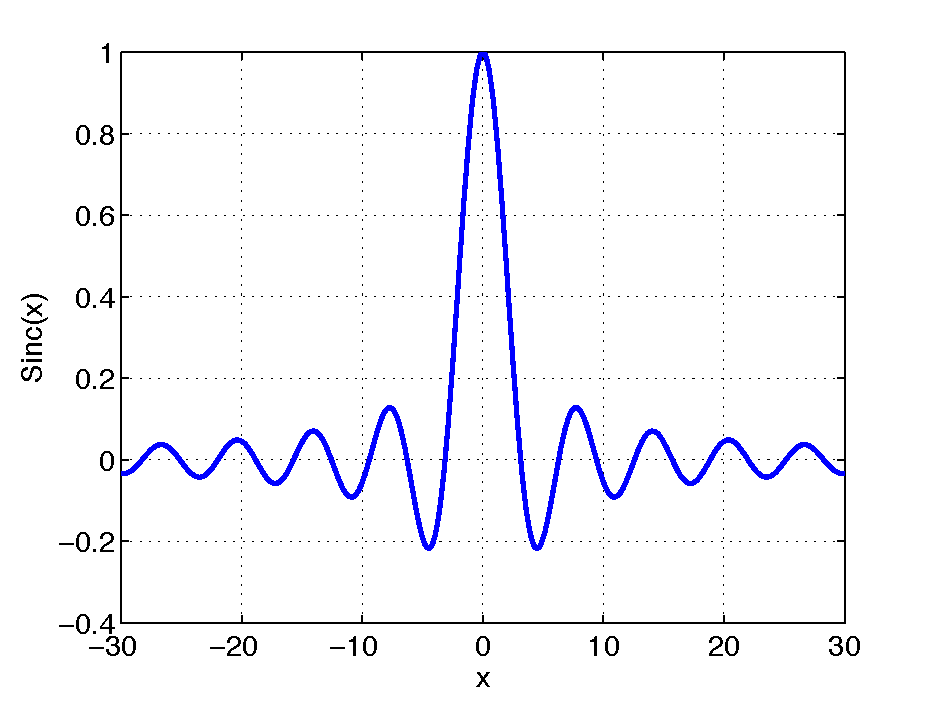
\includegraphics[width=.6\linewidth]{Figures/SincPlot}
%        \caption{Here goes the caption.}
%        \label{fig:Sinc}
%    \end{center}
%\end{figure}
%Figure~\ref{fig:Sinc} shows a shows a plot of the function $\sin(x)/x$. 
%
%If I need to make a simple diagram, I use powerpoint and select the drawing and save it as a pdf. For example, look at Figure~\ref{fig:MechaSys}.
%\begin{figure}[ht]
%    \begin{center}
%        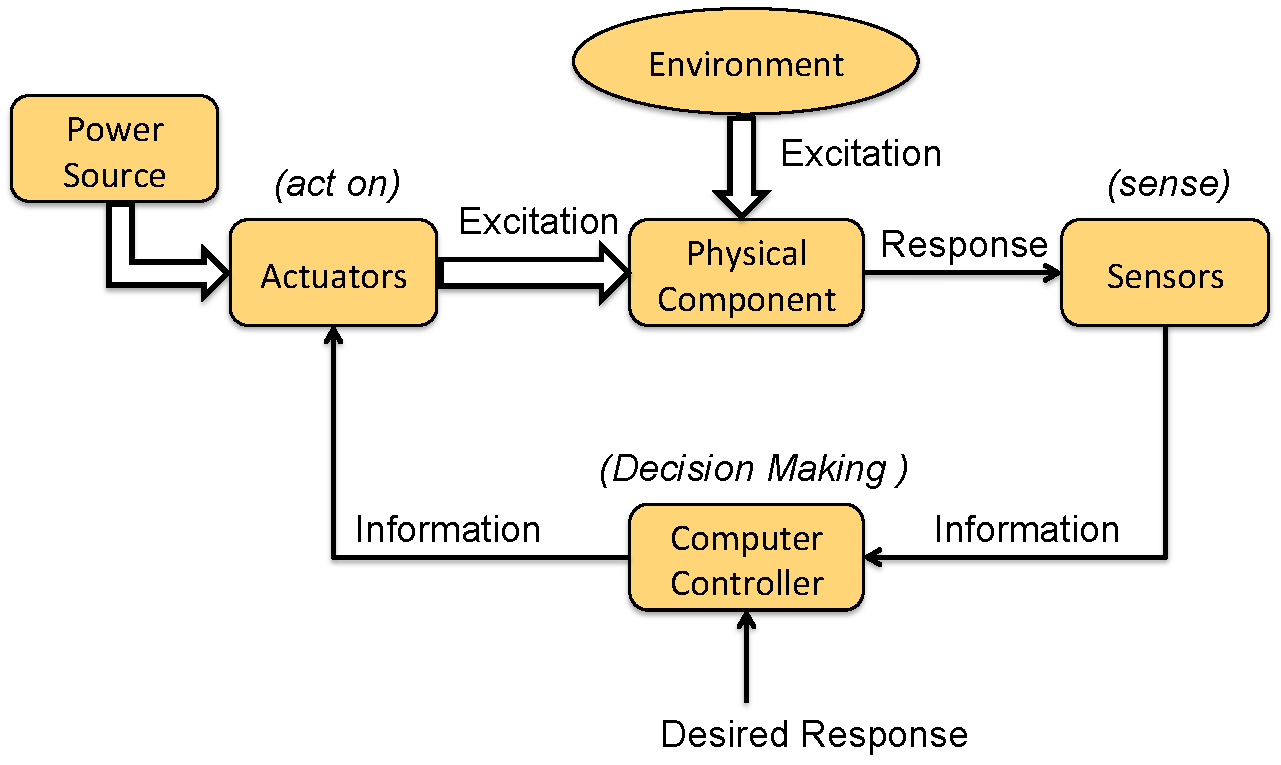
\includegraphics[width=.6\linewidth]{Figures/MechaSys}
%        \caption{Here goes the caption.}
%        \label{fig:MechaSys}
%    \end{center}
%\end{figure}
%%%%%%%%
%\newpage
%\subsection{Lists}
%To create lists use the environments \verb|itemize|, \verb|enumerate|, or \verb|description|
%
%The following is generated using \emph{itemize}
%\begin{itemize}
%    \item This is item 1 
%    \item This is item 2
%\end{itemize}
%%
%The following is generated using \emph{enumerate}
%\begin{enumerate}[1)]
%    \item This is item 1 
%    \begin{enumerate}[a)]
%        \item Subitem a
%        \item Subitem b
%        \begin{enumerate}[i)]
%            \item Subsubitem i
%            \item Subsubitem ii
%        \end{enumerate}
%    \end{enumerate}
%    \item This is item 2
%\end{enumerate}
%%
%The following is generated using \emph{description}
%\begin{description}
%    \item[foo)] This is item 1 
%    \item[bar)] This is item 2
%\end{description}
%
%\subsection{Code listings}
%
%To include a syntax-highlighted code listing, you can use the \emph{listings} package. The default options are specified by the \verb|\lstset| command. There are 3 main commands, all of which can include options to override the defaults:
%\begin{enumerate}
%    \item \verb|\lstinline|: Command for including code fragments inline with the text, as an alternative to \verb|\verb|. For example, we might describe function prototypes such as \lstinline[language=C,breaklines=true]|int main(int argc, char *argv[])|.
%    \item \verb|\begin{lstlisting}|,\ldots,\verb|\end{lstlisting}|: Environment for including a source code listing---embedded in the LaTeX source---in a box or floating environment. An example is shown in Listing~\ref{lst:sqrt}.
%    \item \verb|\lstinputlisting|: Command for including a source code listing---loaded from an external file---in a box or floating environment. This method is preferred over including the code source within the LaTeX file, since the code and its documentation can always be kept in sync. An example is shown in Listing~\ref{lst:matlabserial}.
%\end{enumerate}
%
%\begin{lstlisting}[
%    language=C,
%    float=h,
%    numbers=none,
%    xleftmargin=1cm,
%    frame=none,
%    caption={A winning entry from the 16th International Obfuscated C Code Contest, that computes the square root of its input.\label{lst:sqrt}}
%    ]
%#include <stdio.h>
%int l;int main(int o,char **O,
%int I){char c,*D=O[1];if(o>0){
%for(l=0;D[l              ];D[l
%++]-=10){D   [l++]-=120;D[l]-=
%110;while   (!main(0,O,l))D[l]
%+=   20;   putchar((D[l]+1032)
%/20   )   ;}putchar(10);}else{
%c=o+     (D[I]+82)%10-(I>l/2)*
%(D[I-l+I]+72)/10-9;D[I]+=I<0?0
%:!(o=main(c/10,O,I-1))*((c+999
%)%10-(D[I]+92)%10);}return o;}
%\end{lstlisting}
%
%\lstinputlisting[
%    language=Matlab,
%    float=h,
%    numbers=left,
%    xleftmargin=1cm,
%    frame=shadowbox,
%    caption={Matlab serial communication example.\label{lst:matlabserial}},
%    morekeywords={try,catch}
%    ]{Code/serialtest.m}
%
 %%%%%%%%%%%%%%%%%%%%%%%%%%%%%%%
\NewSection{References and Citations}\label{sec:RefCite}
% To generate the bibliography look at the end of this document in .tex file. To make reference to the bibliography use the commands \verb|\citet{}| and \verb|\citep{}| \citep{strunk2007elements}. You can combine more than one reference in a single citation \citep{troyka1999simon, jay1995write}.

% True \cite{TFwebsite2}
% \citet{TFwebsite2}
% \cit
% %%%%%%%%%%%%%%%%%%%%%%%%%%%%%%%%
% \bibliographystyle{ieeetr}%harvard}
% \bibliography{chris} % This is the .bib file where the bibliography database is stored
\bibliography{main} 
\bibliographystyle{harvard}

\newpage
\appendix
\NewSection{Full Extracts of Journals}
N/A, email correspondance available on request.

\NewSection{Reflection}
about several of the Engineers Australia 16 competencies.  \flagforreview
I'll write this from the first person perspective.
This project was a whirlwind. Taken over the 2018 S2, 2019 S1 period, including the Christmas Holidays, the project was a learning experience. The outcome I got is barely quantifiable past a common sense guess, but I can take pride in knowing the outcome is quantified and based on the `360 hours' minimum of work to get to that result. I learnt a lot starting with\dots
\subsection{Lessons Learnt}
\begin{itemize}
    \item The Industry - FYP was a squandered opportunity on my part, but almost by my choice in FYP topic. Work was able to provide significant support for implementation, and even the prospect of data collection through engaging with potential customers and stakeholders for different use-cases. Unfortunately, I felt uncomfortable pursing that due to how heavy the time spent in implementing felt.  The lesson learnt is to have not done an Industry FYP without understanding how it'll affect the pathway to the final thesis. 
    \item Implementation drove some technology choices I probably would have been better off without. E.g. I went to a Matlab seminar on how to develop Machine Learning in Matlab. Had I used this, the project could have been more homogenous and focused on the big question around "Acoustic Event Detection/Classification". But to do so means I don't develop the python ML skills needed for 'real world' ML tasks. A lesson learnt is to focus on what is assessable, and to probably have used Matlab to demonstrate I understood the theory, not to learn and demonstrate the actual skills of Industry.
    \item The FYP is a ~10 week full time commitment to meet the 360 hours. I potentially \inlineQuote{wasted} 6 weeks just identifying the question I was trying to answer in the report. If I hadn't elected to do a Industry FYP, this is potentially work that could be better shared between the supervisor and myself.
    \item Smaller Scope, get it done in Part A, expand and write in Part B.
\end{itemize}

The FYP has made me appreciate Subject Matter Expertise. In MCHA3900, I focused heavily on understanding the physical hardware involved in the Hexapod - Matlab, RPi, i2c, Openservo v3, and the physical bot itself. I felt I knew that system well, but I recognised my limited understanding. In comparison to that, I reflect on \textit{how much} I've learnt during this FYP, and to what depth of detail compared to MCHA3900. I think I already knew that when I read it's `MCHA3900 - INTRO TO ROBOTICS', but seeing how that was already a good 200 hours I'm surprised just how much more I've had to delve into this.

On that note, I lastly reflect on the skills I've learnt, and the perspective I've gained in how complex the field is, and how much more there is to learn.


\NewSection{Full Result Output}

\subsection{Binary Classifier}
\begin{lstlisting}
    PS C:\FYP\2019-05-11\extra sensor> .\culled_python.py
    00EABED2-271D-49D8-B599-1D4A09240601.features_labels.csv.gz |X2287-Y2287 / timestamps 2287 / feature_names 225 / label_names 51
    098A72A5-E3E5-4F54-A152-BBDA0DF7B694.features_labels.csv.gz |X9100-Y9100 / timestamps 9100 / feature_names 225 / label_names 51
    0A986513-7828-4D53-AA1F-E02D6DF9561B.features_labels.csv.gz |X13060-Y13060 / timestamps 13060 / feature_names 225 / label_names 51
    0BFC35E2-4817-4865-BFA7-764742302A2D.features_labels.csv.gz |X16168-Y16168 / timestamps 16168 / feature_names 225 / label_names 51
    0E6184E1-90C0-48EE-B25A-F1ECB7B9714E.features_labels.csv.gz |X23689-Y23689 / timestamps 23689 / feature_names 225 / label_names 51
    1155FF54-63D3-4AB2-9863-8385D0BD0A13.features_labels.csv.gz |X26374-Y26374 / timestamps 26374 / feature_names 225 / label_names 51
    11B5EC4D-4133-4289-B475-4E737182A406.features_labels.csv.gz |X35219-Y35219 / timestamps 35219 / feature_names 225 / label_names 51
    136562B6-95B2-483D-88DC-065F28409FD2.features_labels.csv.gz |X41437-Y41437 / timestamps 41437 / feature_names 225 / label_names 51
    1538C99F-BA1E-4EFB-A949-6C7C47701B20.features_labels.csv.gz |X47986-Y47986 / timestamps 47986 / feature_names 225 / label_names 51
    1DBB0F6F-1F81-4A50-9DF4-CD62ACFA4842.features_labels.csv.gz |X55361-Y55361 / timestamps 55361 / feature_names 225 / label_names 51
    24E40C4C-A349-4F9F-93AB-01D00FB994AF.features_labels.csv.gz |X60132-Y60132 / timestamps 60132 / feature_names 225 / label_names 51
    27E04243-B138-4F40-A164-F40B60165CF3.features_labels.csv.gz |X65059-Y65059 / timestamps 65059 / feature_names 225 / label_names 51
    2C32C23E-E30C-498A-8DD2-0EFB9150A02E.features_labels.csv.gz |X73575-Y73575 / timestamps 73575 / feature_names 225 / label_names 51
    33A85C34-CFE4-4732-9E73-0A7AC861B27A.features_labels.csv.gz |X79747-Y79747 / timestamps 79747 / feature_names 225 / label_names 51
    3600D531-0C55-44A7-AE95-A7A38519464E.features_labels.csv.gz |X84950-Y84950 / timestamps 84950 / feature_names 225 / label_names 51
    40E170A7-607B-4578-AF04-F021C3B0384A.features_labels.csv.gz |X92599-Y92599 / timestamps 92599 / feature_names 225 / label_names 51
    481F4DD2-7689-43B9-A2AA-C8772227162B.features_labels.csv.gz |X99290-Y99290 / timestamps 99290 / feature_names 225 / label_names 51
    4E98F91F-4654-42EF-B908-A3389443F2E7.features_labels.csv.gz |X102540-Y102540 / timestamps 102540 / feature_names 225 / label_names 51
    4FC32141-E888-4BFF-8804-12559A491D8C.features_labels.csv.gz |X107519-Y107519 / timestamps 107519 / feature_names 225 / label_names 51
    5119D0F8-FCA8-4184-A4EB-19421A40DE0D.features_labels.csv.gz |X114136-Y114136 / timestamps 114136 / feature_names 225 / label_names 51
    5152A2DF-FAF3-4BA8-9CA9-E66B32671A53.features_labels.csv.gz |X120753-Y120753 / timestamps 120753 / feature_names 225 / label_names 51
    59818CD2-24D7-4D32-B133-24C2FE3801E5.features_labels.csv.gz |X126700-Y126700 / timestamps 126700 / feature_names 225 / label_names 51
    59EEFAE0-DEB0-4FFF-9250-54D2A03D0CF2.features_labels.csv.gz |X134242-Y134242 / timestamps 134242 / feature_names 225 / label_names 51
    5EF64122-B513-46AE-BCF1-E62AAC285D2C.features_labels.csv.gz |X138153-Y138153 / timestamps 138153 / feature_names 225 / label_names 51
    61359772-D8D8-480D-B623-7C636EAD0C81.features_labels.csv.gz |X144232-Y144232 / timestamps 144232 / feature_names 225 / label_names 51
    61976C24-1C50-4355-9C49-AAE44A7D09F6.features_labels.csv.gz |X152962-Y152962 / timestamps 152962 / feature_names 225 / label_names 51
    665514DE-49DC-421F-8DCB-145D0B2609AD.features_labels.csv.gz |X162129-Y162129 / timestamps 162129 / feature_names 225 / label_names 51
    74B86067-5D4B-43CF-82CF-341B76BEA0F4.features_labels.csv.gz |X169427-Y169427 / timestamps 169427 / feature_names 225 / label_names 51
    78A91A4E-4A51-4065-BDA7-94755F0BB3BB.features_labels.csv.gz |X181423-Y181423 / timestamps 181423 / feature_names 225 / label_names 51
    797D145F-3858-4A7F-A7C2-A4EB721E133C.features_labels.csv.gz |X185016-Y185016 / timestamps 185016 / feature_names 225 / label_names 51
    7CE37510-56D0-4120-A1CF-0E23351428D2.features_labels.csv.gz |X194777-Y194777 / timestamps 194777 / feature_names 225 / label_names 51
    7D9BB102-A612-4E2A-8E22-3159752F55D8.features_labels.csv.gz |X196377-Y196377 / timestamps 196377 / feature_names 225 / label_names 51
    8023FE1A-D3B0-4E2C-A57A-9321B7FC755F.features_labels.csv.gz |X205566-Y205566 / timestamps 205566 / feature_names 225 / label_names 51
    806289BC-AD52-4CC1-806C-0CDB14D65EB6.features_labels.csv.gz |X214808-Y214808 / timestamps 214808 / feature_names 225 / label_names 51
    81536B0A-8DBF-4D8A-AC24-9543E2E4C8E0.features_labels.csv.gz |X221215-Y221215 / timestamps 221215 / feature_names 225 / label_names 51
    83CF687B-7CEC-434B-9FE8-00C3D5799BE6.features_labels.csv.gz |X230754-Y230754 / timestamps 230754 / feature_names 225 / label_names 51
    86A4F379-B305-473D-9D83-FC7D800180EF.features_labels.csv.gz |X241492-Y241492 / timestamps 241492 / feature_names 225 / label_names 51
    96A358A0-FFF2-4239-B93E-C7425B901B47.features_labels.csv.gz |X247311-Y247311 / timestamps 247311 / feature_names 225 / label_names 51
    9759096F-1119-4E19-A0AD-6F16989C7E1C.features_labels.csv.gz |X257270-Y257270 / timestamps 257270 / feature_names 225 / label_names 51
    99B204C0-DD5C-4BB7-83E8-A37281B8D769.features_labels.csv.gz |X263308-Y263308 / timestamps 263308 / feature_names 225 / label_names 51
    9DC38D04-E82E-4F29-AB52-B476535226F2.features_labels.csv.gz |X272994-Y272994 / timestamps 272994 / feature_names 225 / label_names 51
    A5A30F76-581E-4757-97A2-957553A2C6AA.features_labels.csv.gz |X274661-Y274661 / timestamps 274661 / feature_names 225 / label_names 51
    A5CDF89D-02A2-4EC1-89F8-F534FDABDD96.features_labels.csv.gz |X280701-Y280701 / timestamps 280701 / feature_names 225 / label_names 51
    A7599A50-24AE-46A6-8EA6-2576F1011D81.features_labels.csv.gz |X284599-Y284599 / timestamps 284599 / feature_names 225 / label_names 51
    A76A5AF5-5A93-4CF2-A16E-62353BB70E8A.features_labels.csv.gz |X292119-Y292119 / timestamps 292119 / feature_names 225 / label_names 51
    B09E373F-8A54-44C8-895B-0039390B859F.features_labels.csv.gz |X300253-Y300253 / timestamps 300253 / feature_names 225 / label_names 51
    B7F9D634-263E-4A97-87F9-6FFB4DDCB36C.features_labels.csv.gz |X309636-Y309636 / timestamps 309636 / feature_names 225 / label_names 51
    B9724848-C7E2-45F4-9B3F-A1F38D864495.features_labels.csv.gz |X317262-Y317262 / timestamps 317262 / feature_names 225 / label_names 51
    BE3CA5A6-A561-4BBD-B7C9-5DF6805400FC.features_labels.csv.gz |X325571-Y325571 / timestamps 325571 / feature_names 225 / label_names 51
    BEF6C611-50DA-4971-A040-87FB979F3FC1.features_labels.csv.gz |X329022-Y329022 / timestamps 329022 / feature_names 225 / label_names 51
    C48CE857-A0DD-4DDB-BEA5-3A25449B2153.features_labels.csv.gz |X334114-Y334114 / timestamps 334114 / feature_names 225 / label_names 51
    CA820D43-E5E2-42EF-9798-BE56F776370B.features_labels.csv.gz |X341979-Y341979 / timestamps 341979 / feature_names 225 / label_names 51
    CCAF77F0-FABB-4F2F-9E24-D56AD0C5A82F.features_labels.csv.gz |X350451-Y350451 / timestamps 350451 / feature_names 225 / label_names 51
    CDA3BBF7-6631-45E8-85BA-EEB416B32A3C.features_labels.csv.gz |X353311-Y353311 / timestamps 353311 / feature_names 225 / label_names 51
    CF722AA9-2533-4E51-9FEB-9EAC84EE9AAC.features_labels.csv.gz |X356926-Y356926 / timestamps 356926 / feature_names 225 / label_names 51
    D7D20E2E-FC78-405D-B346-DBD3FD8FC92B.features_labels.csv.gz |X363136-Y363136 / timestamps 363136 / feature_names 225 / label_names 51
    E65577C1-8D5D-4F70-AF23-B3ADB9D3DBA3.features_labels.csv.gz |X366577-Y366577 / timestamps 366577 / feature_names 225 / label_names 51
    ECECC2AB-D32F-4F90-B74C-E12A1C69BBE2.features_labels.csv.gz |X370107-Y370107 / timestamps 370107 / feature_names 225 / label_names 51
    F50235E0-DD67-4F2A-B00B-1F31ADA998B9.features_labels.csv.gz |X372373-Y372373 / timestamps 372373 / feature_names 225 / label_names 51
    end
    layer sizes
    Fitting 3 folds for each of 30 candidates, totalling 90 fits
    [Parallel(n_jobs=-1)]: Using backend LokyBackend with 4 concurrent workers.
    [Parallel(n_jobs=-1)]: Done  42 tasks      | elapsed: 27.3min
    [Parallel(n_jobs=-1)]: Done  90 out of  90 | elapsed: 53.6min finished
    F-Score: 0.92
    {'solver': 'adam', 'learning_rate': 'adaptive', 'hidden_layer_sizes': (150, 100, 50), 'alpha': 0.03, 'activation': 'tanh'}
    --- Training Metrics ---
    Samples: 8766
    Label: Walking
    TP: 18835024
    TN: 12425049
    Sensors: ['Aud', 'Acc', 'Gyro', 'Loc']
    Features: 7865 features
    --- Performance Metrics ---
    Accuracy: 0.51
    Recall(sensitivity): 0.55
    Precision: 0.55
    Specificity: 0.45
    F-Score: 0.84
    --- Confusion Matrix CLASS 2 ---
    [[2892  657]
     [ 609 3707]]
    --- Training Metrics ---
    Samples: 4973
    Label: Walking
    TP: 167919
    TN: 2718675
    Sensors: ['Aud', 'Acc', 'Gyro', 'Loc']
    Features: 2158 features
    --- Performance Metrics ---
    Accuracy: 0.62
    Recall(sensitivity): 0.35
    Precision: 0.10
    Specificity: 0.65
    F-Score: 0.80
    --- Confusion Matrix CLASS 2 ---
    [[1400  535]
     [   5  218]]
    layer sizes
    Fitting 3 folds for each of 30 candidates, totalling 90 fits
    [Parallel(n_jobs=-1)]: Using backend LokyBackend with 4 concurrent workers.
    [Parallel(n_jobs=-1)]: Done  42 tasks      | elapsed: 25.6min
    [Parallel(n_jobs=-1)]: Done  90 out of  90 | elapsed: 42.9min finished
    F-Score: 0.82
    {'solver': 'adam', 'learning_rate': 'constant', 'hidden_layer_sizes': (300,), 'alpha': 0.001, 'activation': 'relu'}
    --- Training Metrics ---
    Samples: 8766
    Label: Walking
    TP: 21205444
    TN: 10764288
    Sensors: ['Aud']
    Features: 7898 features
    --- Performance Metrics ---
    Accuracy: 0.51
    Recall(sensitivity): 0.61
    Precision: 0.56
    Specificity: 0.39
    F-Score: 0.76
    --- Confusion Matrix CLASS 2 ---
    [[2366 1138]
     [ 706 3688]]
    --- Training Metrics ---
    Samples: 4973
    Label: Walking
    TP: 233481
    TN: 2149785
    Sensors: ['Aud']
    Features: 2158 features
    --- Performance Metrics ---
    Accuracy: 0.51
    Recall(sensitivity): 0.49
    Precision: 0.10
    Specificity: 0.51
    F-Score: 0.69
    --- Confusion Matrix CLASS 2 ---
    [[1109  826]
     [   2  221]]
\end{lstlisting}
\subsection{Multi-label Classifier}
\begin{lstlisting}
00EABED2-271D-49D8-B599-1D4A09240601.features_labels.csv.gz |X2287-Y2287 / timestamps 2287 / feature_names 225 / label_names 51
098A72A5-E3E5-4F54-A152-BBDA0DF7B694.features_labels.csv.gz |X9100-Y9100 / timestamps 9100 / feature_names 225 / label_names 51
0A986513-7828-4D53-AA1F-E02D6DF9561B.features_labels.csv.gz |X13060-Y13060 / timestamps 13060 / feature_names 225 / label_names 51
0BFC35E2-4817-4865-BFA7-764742302A2D.features_labels.csv.gz |X16168-Y16168 / timestamps 16168 / feature_names 225 / label_names 51
0E6184E1-90C0-48EE-B25A-F1ECB7B9714E.features_labels.csv.gz |X23689-Y23689 / timestamps 23689 / feature_names 225 / label_names 51
1155FF54-63D3-4AB2-9863-8385D0BD0A13.features_labels.csv.gz |X26374-Y26374 / timestamps 26374 / feature_names 225 / label_names 51
11B5EC4D-4133-4289-B475-4E737182A406.features_labels.csv.gz |X35219-Y35219 / timestamps 35219 / feature_names 225 / label_names 51
136562B6-95B2-483D-88DC-065F28409FD2.features_labels.csv.gz |X41437-Y41437 / timestamps 41437 / feature_names 225 / label_names 51
1538C99F-BA1E-4EFB-A949-6C7C47701B20.features_labels.csv.gz |X47986-Y47986 / timestamps 47986 / feature_names 225 / label_names 51
1DBB0F6F-1F81-4A50-9DF4-CD62ACFA4842.features_labels.csv.gz |X55361-Y55361 / timestamps 55361 / feature_names 225 / label_names 51
24E40C4C-A349-4F9F-93AB-01D00FB994AF.features_labels.csv.gz |X60132-Y60132 / timestamps 60132 / feature_names 225 / label_names 51
27E04243-B138-4F40-A164-F40B60165CF3.features_labels.csv.gz |X65059-Y65059 / timestamps 65059 / feature_names 225 / label_names 51
2C32C23E-E30C-498A-8DD2-0EFB9150A02E.features_labels.csv.gz |X73575-Y73575 / timestamps 73575 / feature_names 225 / label_names 51
33A85C34-CFE4-4732-9E73-0A7AC861B27A.features_labels.csv.gz |X79747-Y79747 / timestamps 79747 / feature_names 225 / label_names 51
3600D531-0C55-44A7-AE95-A7A38519464E.features_labels.csv.gz |X84950-Y84950 / timestamps 84950 / feature_names 225 / label_names 51
40E170A7-607B-4578-AF04-F021C3B0384A.features_labels.csv.gz |X92599-Y92599 / timestamps 92599 / feature_names 225 / label_names 51
481F4DD2-7689-43B9-A2AA-C8772227162B.features_labels.csv.gz |X99290-Y99290 / timestamps 99290 / feature_names 225 / label_names 51
4E98F91F-4654-42EF-B908-A3389443F2E7.features_labels.csv.gz |X102540-Y102540 / timestamps 102540 / feature_names 225 / label_names 51
4FC32141-E888-4BFF-8804-12559A491D8C.features_labels.csv.gz |X107519-Y107519 / timestamps 107519 / feature_names 225 / label_names 51
5119D0F8-FCA8-4184-A4EB-19421A40DE0D.features_labels.csv.gz |X114136-Y114136 / timestamps 114136 / feature_names 225 / label_names 51
5152A2DF-FAF3-4BA8-9CA9-E66B32671A53.features_labels.csv.gz |X120753-Y120753 / timestamps 120753 / feature_names 225 / label_names 51
59818CD2-24D7-4D32-B133-24C2FE3801E5.features_labels.csv.gz |X126700-Y126700 / timestamps 126700 / feature_names 225 / label_names 51
59EEFAE0-DEB0-4FFF-9250-54D2A03D0CF2.features_labels.csv.gz |X134242-Y134242 / timestamps 134242 / feature_names 225 / label_names 51
5EF64122-B513-46AE-BCF1-E62AAC285D2C.features_labels.csv.gz |X138153-Y138153 / timestamps 138153 / feature_names 225 / label_names 51
61359772-D8D8-480D-B623-7C636EAD0C81.features_labels.csv.gz |X144232-Y144232 / timestamps 144232 / feature_names 225 / label_names 51
61976C24-1C50-4355-9C49-AAE44A7D09F6.features_labels.csv.gz |X152962-Y152962 / timestamps 152962 / feature_names 225 / label_names 51
665514DE-49DC-421F-8DCB-145D0B2609AD.features_labels.csv.gz |X162129-Y162129 / timestamps 162129 / feature_names 225 / label_names 51
74B86067-5D4B-43CF-82CF-341B76BEA0F4.features_labels.csv.gz |X169427-Y169427 / timestamps 169427 / feature_names 225 / label_names 51
78A91A4E-4A51-4065-BDA7-94755F0BB3BB.features_labels.csv.gz |X181423-Y181423 / timestamps 181423 / feature_names 225 / label_names 51
797D145F-3858-4A7F-A7C2-A4EB721E133C.features_labels.csv.gz |X185016-Y185016 / timestamps 185016 / feature_names 225 / label_names 51
7CE37510-56D0-4120-A1CF-0E23351428D2.features_labels.csv.gz |X194777-Y194777 / timestamps 194777 / feature_names 225 / label_names 51
7D9BB102-A612-4E2A-8E22-3159752F55D8.features_labels.csv.gz |X196377-Y196377 / timestamps 196377 / feature_names 225 / label_names 51
8023FE1A-D3B0-4E2C-A57A-9321B7FC755F.features_labels.csv.gz |X205566-Y205566 / timestamps 205566 / feature_names 225 / label_names 51
806289BC-AD52-4CC1-806C-0CDB14D65EB6.features_labels.csv.gz |X214808-Y214808 / timestamps 214808 / feature_names 225 / label_names 51
81536B0A-8DBF-4D8A-AC24-9543E2E4C8E0.features_labels.csv.gz |X221215-Y221215 / timestamps 221215 / feature_names 225 / label_names 51
83CF687B-7CEC-434B-9FE8-00C3D5799BE6.features_labels.csv.gz |X230754-Y230754 / timestamps 230754 / feature_names 225 / label_names 51
86A4F379-B305-473D-9D83-FC7D800180EF.features_labels.csv.gz |X241492-Y241492 / timestamps 241492 / feature_names 225 / label_names 51
96A358A0-FFF2-4239-B93E-C7425B901B47.features_labels.csv.gz |X247311-Y247311 / timestamps 247311 / feature_names 225 / label_names 51
9759096F-1119-4E19-A0AD-6F16989C7E1C.features_labels.csv.gz |X257270-Y257270 / timestamps 257270 / feature_names 225 / label_names 51
99B204C0-DD5C-4BB7-83E8-A37281B8D769.features_labels.csv.gz |X263308-Y263308 / timestamps 263308 / feature_names 225 / label_names 51
9DC38D04-E82E-4F29-AB52-B476535226F2.features_labels.csv.gz |X272994-Y272994 / timestamps 272994 / feature_names 225 / label_names 51
A5A30F76-581E-4757-97A2-957553A2C6AA.features_labels.csv.gz |X274661-Y274661 / timestamps 274661 / feature_names 225 / label_names 51
A5CDF89D-02A2-4EC1-89F8-F534FDABDD96.features_labels.csv.gz |X280701-Y280701 / timestamps 280701 / feature_names 225 / label_names 51
A7599A50-24AE-46A6-8EA6-2576F1011D81.features_labels.csv.gz |X284599-Y284599 / timestamps 284599 / feature_names 225 / label_names 51
A76A5AF5-5A93-4CF2-A16E-62353BB70E8A.features_labels.csv.gz |X292119-Y292119 / timestamps 292119 / feature_names 225 / label_names 51
B09E373F-8A54-44C8-895B-0039390B859F.features_labels.csv.gz |X300253-Y300253 / timestamps 300253 / feature_names 225 / label_names 51
B7F9D634-263E-4A97-87F9-6FFB4DDCB36C.features_labels.csv.gz |X309636-Y309636 / timestamps 309636 / feature_names 225 / label_names 51
B9724848-C7E2-45F4-9B3F-A1F38D864495.features_labels.csv.gz |X317262-Y317262 / timestamps 317262 / feature_names 225 / label_names 51
BE3CA5A6-A561-4BBD-B7C9-5DF6805400FC.features_labels.csv.gz |X325571-Y325571 / timestamps 325571 / feature_names 225 / label_names 51
BEF6C611-50DA-4971-A040-87FB979F3FC1.features_labels.csv.gz |X329022-Y329022 / timestamps 329022 / feature_names 225 / label_names 51
C48CE857-A0DD-4DDB-BEA5-3A25449B2153.features_labels.csv.gz |X334114-Y334114 / timestamps 334114 / feature_names 225 / label_names 51
CA820D43-E5E2-42EF-9798-BE56F776370B.features_labels.csv.gz |X341979-Y341979 / timestamps 341979 / feature_names 225 / label_names 51
CCAF77F0-FABB-4F2F-9E24-D56AD0C5A82F.features_labels.csv.gz |X350451-Y350451 / timestamps 350451 / feature_names 225 / label_names 51
CDA3BBF7-6631-45E8-85BA-EEB416B32A3C.features_labels.csv.gz |X353311-Y353311 / timestamps 353311 / feature_names 225 / label_names 51
CF722AA9-2533-4E51-9FEB-9EAC84EE9AAC.features_labels.csv.gz |X356926-Y356926 / timestamps 356926 / feature_names 225 / label_names 51
D7D20E2E-FC78-405D-B346-DBD3FD8FC92B.features_labels.csv.gz |X363136-Y363136 / timestamps 363136 / feature_names 225 / label_names 51
E65577C1-8D5D-4F70-AF23-B3ADB9D3DBA3.features_labels.csv.gz |X366577-Y366577 / timestamps 366577 / feature_names 225 / label_names 51
ECECC2AB-D32F-4F90-B74C-E12A1C69BBE2.features_labels.csv.gz |X370107-Y370107 / timestamps 370107 / feature_names 225 / label_names 51
F50235E0-DD67-4F2A-B00B-1F31ADA998B9.features_labels.csv.gz |X372373-Y372373 / timestamps 372373 / feature_names 225 / label_names 51
end
layer sizes
Fitting 3 folds for each of 30 candidates, totalling 90 fits
[Parallel(n_jobs=-1)]: Using backend LokyBackend with 4 concurrent workers.
F-Score: 0.60
{'solver': 'adam', 'learning_rate': 'invscaling', 'hidden_layer_sizes': (151, 52, 26), 'alpha': 0.07, 'activation': 'tanh'}
----------
----------
--- Training Metrics ---
Samples: 7891
Label: 2:20
TP: 10706
TN: 132399
Sensors: ['Aud', 'Acc', 'Gyro', 'Loc']
Features: 7891 features
--- Performance Metrics ---
Accuracy: 0.95
Recall(sensitivity): 0.73
Precision: 0.79
Specificity: 0.98
F-Score: 0.75
--- Confusion Matrix CLASS 2 ---
[[2874  633]
 [ 709 3675]]
--- Confusion Matrix CLASS 3 ---
[[7876    0]
 [  15    0]]
--- Confusion Matrix CLASS 4 ---
[[7812    2]
 [  45   32]]
--- Confusion Matrix CLASS 5 ---
[[6639  214]
 [ 178  860]]
--- Confusion Matrix CLASS 6 ---
[[7822    5]
 [  60    4]]
--- Confusion Matrix CLASS 7 ---
[[7801    8]
 [  71   11]]
--- Confusion Matrix CLASS 8 ---
[[7811    0]
 [  80    0]]
--- Confusion Matrix CLASS 9 ---
[[7102  132]
 [ 292  365]]
--- Confusion Matrix CLASS 10 ---
[[4375  585]
 [ 603 2328]]
--- Confusion Matrix CLASS 11 ---
[[6234  362]
 [ 532  763]]
--- Confusion Matrix CLASS 12 ---
[[7795   14]
 [  65   17]]
--- Confusion Matrix CLASS 13 ---
[[7867    0]
 [  24    0]]
--- Confusion Matrix CLASS 14 ---
[[7757   36]
 [  72   26]]
--- Confusion Matrix CLASS 15 ---
[[7853    1]
 [  36    1]]
--- Confusion Matrix CLASS 16 ---
[[5155  511]
 [ 411 1814]]
--- Confusion Matrix CLASS 17 ---
[[7861    0]
 [  30    0]]
--- Confusion Matrix CLASS 18 ---
[[6297  266]
 [ 631  697]]
--- Confusion Matrix CLASS 19 ---
[[7757    5]
 [  85   44]]
--- Confusion Matrix CLASS 20 ---
[[7711   31]
 [  80   69]]
----------
----------
--- Training Metrics ---
Samples: 2158
Label: 2:20
TP: 537
TN: 36996
Sensors: ['Aud', 'Acc', 'Gyro', 'Loc']
Features: 2158 features
--- Performance Metrics ---
Accuracy: 0.92
Recall(sensitivity): 0.43
Precision: 0.16
Specificity: 0.93
F-Score: 0.42
--- Confusion Matrix CLASS 2 ---
[[1374  561]
 [   7  216]]
--- Confusion Matrix CLASS 3 ---
[[2158]]
--- Confusion Matrix CLASS 4 ---
[[2156    2]
 [   0    0]]
--- Confusion Matrix CLASS 5 ---
[[1998  160]
 [   0    0]]
--- Confusion Matrix CLASS 6 ---
[[2041  117]
 [   0    0]]
--- Confusion Matrix CLASS 7 ---
[[2155    3]
 [   0    0]]
--- Confusion Matrix CLASS 8 ---
[[2158]]
--- Confusion Matrix CLASS 9 ---
[[1685  473]
 [   0    0]]
--- Confusion Matrix CLASS 10 ---
[[1502  656]
 [   0    0]]
--- Confusion Matrix CLASS 11 ---
[[2024  134]
 [   0    0]]
--- Confusion Matrix CLASS 12 ---
[[2125   33]
 [   0    0]]
--- Confusion Matrix CLASS 13 ---
[[2158]]
--- Confusion Matrix CLASS 14 ---
[[2011    0]
 [  89   58]]
--- Confusion Matrix CLASS 15 ---
[[2154    4]
 [   0    0]]
--- Confusion Matrix CLASS 16 ---
[[1731  427]
 [   0    0]]
--- Confusion Matrix CLASS 17 ---
[[2158]]
--- Confusion Matrix CLASS 18 ---
[[1096  184]
 [ 615  263]]
--- Confusion Matrix CLASS 19 ---
[[2154    4]
 [   0    0]]
--- Confusion Matrix CLASS 20 ---
[[2158]]
layer sizes

 ------ REMOVING  --- SUPPLEMENTARY  --- DATA --- ---
 
F-Score: 0.42
----------
----------
--- Training Metrics ---
Samples: 7903
Label: 2:20
TP: 9233
TN: 132687
Sensors: ['Aud']
Features: 7903 features
--- Performance Metrics ---
Accuracy: 0.95
Recall(sensitivity): 0.63
Precision: 0.76
Specificity: 0.98
F-Score: 0.67
--- Confusion Matrix CLASS 2 ---
[[2364 1126]
 [ 691 3722]]
--- Confusion Matrix CLASS 3 ---
[[7891    0]
 [  12    0]]
--- Confusion Matrix CLASS 4 ---
[[7828    2]
 [  68    5]]
--- Confusion Matrix CLASS 5 ---
[[6744  160]
 [ 306  693]]
--- Confusion Matrix CLASS 6 ---
[[7848    1]
 [  47    7]]
--- Confusion Matrix CLASS 7 ---
[[7822    0]
 [  81    0]]
--- Confusion Matrix CLASS 8 ---
[[7810    0]
 [  93    0]]
--- Confusion Matrix CLASS 9 ---
[[7133  100]
 [ 453  217]]
--- Confusion Matrix CLASS 10 ---
[[4610  489]
 [ 833 1971]]
--- Confusion Matrix CLASS 11 ---
[[6297  255]
 [ 807  544]]
--- Confusion Matrix CLASS 12 ---
[[7813    2]
 [  88    0]]
--- Confusion Matrix CLASS 13 ---
[[7881    0]
 [  22    0]]
--- Confusion Matrix CLASS 14 ---
[[7798    7]
 [  92    6]]
--- Confusion Matrix CLASS 15 ---
[[7865    0]
 [  38    0]]
--- Confusion Matrix CLASS 16 ---
[[5344  405]
 [ 658 1496]]
--- Confusion Matrix CLASS 17 ---
[[7860    0]
 [  43    0]]
--- Confusion Matrix CLASS 18 ---
[[6274  314]
 [ 813  502]]
--- Confusion Matrix CLASS 19 ---
[[7784    8]
 [ 102    9]]
--- Confusion Matrix CLASS 20 ---
[[7721   12]
 [ 109   61]]
----------
----------
--- Training Metrics ---
Samples: 2158
Label: 2:20
TP: 380
TN: 37523
Sensors: ['Aud']
Features: 2158 features
--- Performance Metrics ---
Accuracy: 0.92
Recall(sensitivity): 0.30
Precision: 0.15
Specificity: 0.94
F-Score: 0.29
--- Confusion Matrix CLASS 2 ---
[[1307  628]
 [  12  211]]
--- Confusion Matrix CLASS 3 ---
[[2158]]
--- Confusion Matrix CLASS 4 ---
[[2158]]
--- Confusion Matrix CLASS 5 ---
[[1845  313]
 [   0    0]]
--- Confusion Matrix CLASS 6 ---
[[2127   31]
 [   0    0]]
--- Confusion Matrix CLASS 7 ---
[[2158]]
--- Confusion Matrix CLASS 8 ---
[[2158]]
--- Confusion Matrix CLASS 9 ---
[[2139   19]
 [   0    0]]
--- Confusion Matrix CLASS 10 ---
[[1389  769]
 [   0    0]]
--- Confusion Matrix CLASS 11 ---
[[2156    2]
 [   0    0]]
--- Confusion Matrix CLASS 12 ---
[[2149    9]
 [   0    0]]
--- Confusion Matrix CLASS 13 ---
[[2158]]
--- Confusion Matrix CLASS 14 ---
[[2009    2]
 [ 133   14]]
--- Confusion Matrix CLASS 15 ---
[[2158]]
--- Confusion Matrix CLASS 16 ---
[[1780  378]
 [   0    0]]
--- Confusion Matrix CLASS 17 ---
[[2158]]
--- Confusion Matrix CLASS 18 ---
[[1201   79]
 [ 723  155]]
--- Confusion Matrix CLASS 19 ---
[[2157    1]
 [   0    0]]
--- Confusion Matrix CLASS 20 ---
[[2158]]
\end{lstlisting}

\NewSection{Dataset Feature Importance}\label{apx:FeatureImportance}
\fFigure{feature_important_just_audio2.png}{A Random Tree Classifier was used to evaluate feaure importance, during the design phase of the main classifier. Features were Audio (26 bins)}{0.5}

\fFigure{feature_important_just_accel.png}{A Random Tree Classifier was used to evaluate feaure importance, during the design phase of the main classifier. Features were Accelerometer(26)}{0.5}

\fFigure{feature_important_just_Gyro.png}{A Random Tree Classifier was used to evaluate feaure importance, during the design phase of the main classifier. Features were Gyroscope(26)}{0.5}

\fFigure{feature_important_just_GPS2.png}{A Random Tree Classifier was used to evaluate feaure importance, during the design phase of the main classifier. Features were GPS (16)}{0.5}

\NewSection{Trade-Review of "Online vs Offline" processing}\label{sec:TradeReview}


\NewSection{GridSearch Attempts}\label{apx:GSAttempt}
This shows how a Grid Search was used for hyperparameter optimisation. In particular, this is an example of an iteritive process where the grid was manually narrowed and precision increase. 
\begin{lstlisting}
    parameters={'hidden_layer_sizes': [(145,), (147,), (149,), (151,), (153)],
                'alpha': [0.09, 0.11, 0.13, 0.15, 0.17, 0.19]}
    mlpc = MLPClassifier(verbose=False, early_stopping=True, learning_rate='adaptive',max_iter=1000)
    clf = GridSearchCV(estimator=mlpc, scoring='f1',param_grid=parameters,n_jobs=-1,verbose=1,cv=3);
    clf.fit(X_train,y);
    print(clf.score(X_train, y))
    print(clf.best_params_)
\end{lstlisting}
\begin{lstlisting}
    Fitting 3 folds for each of 30 candidates, totalling 90 fits
    [Parallel(n_jobs=-1)]: Using backend LokyBackend with 4 concurrent workers.
    [Parallel(n_jobs=-1)]: Done  42 tasks      | elapsed:  7.8min
    [Parallel(n_jobs=-1)]: Done  90 out of  90 | elapsed: 14.4min finished
    0.8249400479616308
    {'alpha': 0.11, 'hidden_layer_sizes': (151,)}
\end{lstlisting}


\NewSection{Table of ExtraSensory Labels}\label{apx:ExtraSensoryLabels}
\begin{table}[h]
\begin{center}  
\caption{ExtraSensory Labels \cite{Vaizman2017}}\label{tab:ExtraSensoryLabels}
\begin{tabular}{ll}
    \hline\hline
\# & Label Description            \\ \hline 
1  & LYING\_DOWN                  \\
2  & SITTING                      \\
3  & FIX\_walking                 \\
4  & FIX\_running                 \\
5  & BICYCLING                    \\
6  & SLEEPING                     \\
7  & LAB\_WORK                    \\
8  & IN\_CLASS                    \\
9  & IN\_A\_MEETING               \\
10 & LOC\_main\_workplace         \\
11 & OR\_indoors                  \\
12 & OR\_outside                  \\
13 & IN\_A\_CAR                   \\
14 & ON\_A\_BUS                   \\
15 & DRIVE\_-\_I\_M\_THE\_DRIVER  \\
16 & DRIVE\_-\_I\_M\_A\_PASSENGER \\
17 & LOC\_home                    \\
18 & FIX\_restaurant              \\
19 & PHONE\_IN\_POCKET            \\
20 & OR\_exercise                 \\
21 & COOKING                      \\
22 & SHOPPING                     \\
23 & STROLLING                    \\
24 & DRINKING\_\_ALCOHOL\_        \\
25 & BATHING\_-\_SHOWER           \\
26 & CLEANING                     \\
27 & DOING\_LAUNDRY               \\
28 & WASHING\_DISHES              \\
29 & WATCHING\_TV                 \\
30 & SURFING\_THE\_INTERNET       \\
31 & AT\_A\_PARTY                 \\
32 & AT\_A\_BAR                   \\
33 & LOC\_beach                   \\
34 & SINGING                      \\
35 & TALKING                      \\
36 & COMPUTER\_WORK               \\
37 & EATING                       \\
38 & TOILET                       \\
39 & GROOMING                     \\
40 & DRESSING                     \\
41 & AT\_THE\_GYM                 \\
42 & STAIRS\_-\_GOING\_UP         \\
43 & STAIRS\_-\_GOING\_DOWN       \\
44 & ELEVATOR                     \\
45 & OR\_standing                 \\
46 & AT\_SCHOOL                   \\
47 & PHONE\_IN\_HAND              \\
48 & PHONE\_IN\_BAG               \\
49 & PHONE\_ON\_TABLE             \\
50 & WITH\_CO-WORKERS             \\
51 & WITH\_FRIENDS                \\ \hline 
\end{tabular}    
\end{center}
\end{table}
%%%%%%%%%%%%%%%%%%%%%%%%%%%%%%%%%%%%%%%%%%%%%%%%%%%%%%%%%%%%%%%%%%%%%%%%%%%%%%%%%%%%%%%%%%%%%%%%%%%%%%%%%%%%%%%%%%%%%%%%%%%%%%%%%%%%%%%%%%%%%%%%%%%%%%%%%%%%%%%%%%%%%%%%%%%%%%%%%%%%%%%%%%%%%%%%%%%%%%%%%%%%%%%%%%%%%%%%%%%%%%%%%%%%%%%%%%%%%%%%%%%%%%%%%%%%%%%%%%%%%%%%%%%%%%%%%%%%%%%%%%%%%%%%%%%%%%%%%%%%%%%%%%%%%%%%%%%%%%%%%%%%%%%%%%%%%%%%%%%%%%%%%%%%%%%%%%%%%%%%%%%%%%%%%%%%%%%%%%%%%%%%%%%%%%%%%%%%%%%%%%%%%%%%%%%%%%%%%%%%%%%%%%%%%%%%%%%%%%%%%%%%%%%%%%%%%%%%%%%%%%%%%%%%%%%%%%%%%%%%%%%%%%%%%%%%%%%%%%%%%%%%%%%%%%%%%%%%%%%%%%%%%%%%%%%%%%%%%%%%%%%%%%%%%%%%%%%%%%%%%%%%%%%%%%%%%%%%%%%%%%%%%%%%%%%%%%%%%%%%%%%%%%%%%%%%%%%%%%%%%%%%%%%%%%%%%%%%%%%%%%%%%%%%%%%%%%%%%%%%
%%%%%%%%%%%%%%%%%%%%%%%%%%%%%%%%%%%%%%%%%%%%%%%%%%%%%%%%%%%%%%%%%%%%%%%%%%%%%%%%%%%%%%%%%%%%%%%%%%%%%%%%%%%%%%%%%%%%%%%%%%%%%%%%%%%%%%%%%%%%%%%%%%%%%%%%%%%%%%%%%%%%%%%%%%%%%%%%%%%%%%%%%%%%%%%%%%%%%%%%%%%%%%%%%%%%%%%%%%%%%%%%%%%%%%%%%%%%%%%%%%%%%%%%%%%%%%%%%%%%%%%%%%%%%%%%%%%%%%%%%%%%%%%%%%%%%%%%%%%%%%%%%%%%%%%%%%%%%%%%%%%%%%%%%%%%%%%%%%%%%%%%%%%%%%%%%%%%%%%%%%%%%%%%%%%%%%%%%%%%%%%%%%%%%%%%%%%%%%%%%%%%%%%%%%%%%%%%%%%%%%%%%%%%%%%%%%%%%%%%%%%%%%%%%%%%%%%%%%%%%%%%%%%%%%%%%%%%%%%%%%%%%%%%%%%%%%%%%%%%%%%%%%%%%%%%%%%%%%%%%%%%%%%%%%%%%%%%%%%%%%%%%%%%%%%%%%%%%%%%%%%%%%%%%%%%%%%%%%%%%%%%%%%%%%%%%%%%%%%%%%%%%%%%%%%%%%%%%%%%%%%%%%%%%%%%%%%%%%%%%%%%%%%%%%%%%%%%%%%%

% \NewSection{Writing you're not sure if you want to keep}






% \subsection{Development Tools and Technologies}
% Windows 10, i7-7500U and GeForce 940MX, Nvidia 1080Ti, VS Code, LaTeX, Python, Matlab, sklearn, numpy, ExtraSensory dataset, git.

% Visual Studio was used for developing the Python project

% \subsection{Discussion on practical aspects of IMU and Audio}

% \begin{itemize}
%     \item I'm not sure if it's practical to try and be recording IMU plus audio
%     \item It's a case of POV; if you can record IMU, you can also record audio from the POV of your user. This theoretically suggests a higher fidelity in classification, especially in determining whether an event was local (POV) or whether it was an external event (someone else)
%     \item whilst IMU is helpful, the level of understanding
% \end{itemize}



% \subsection{Nearest Neighbour}
% Nearest Neighbour was chosen as a classification method to test against, and evaluate the other methods. Nearest Neighbour would not be used as a primary method as does not generalise well\citationneeded \footnote{https://scikit-learn.org/stable/modules/neighbors.html}



% ciation:

% Vaizman2017a	
% Vaizman, Y., Ellis, K., and Lanckriet, G. "Recognizing Detailed Human Context In-the-Wild from Smartphones and Smartwatches". IEEE Pervasive Computing, vol. 16, no. 4, October-December 2017, pp. 62-74. doi:10.1109/MPRV.2017.3971131
% *Cite this paper if you use the ExtraSensory Dataset for any publication!




% sounds like dropout is great for making sure accelerometer data is used

% Dropout

% Unlike these methods mentioned above, dropout in my understanding is tricky but practical. Like the figure shown below, the dropout will randomly mute some neurons in the neural network and we therefore have a sparse network which hugely decreases the possibility of overfitting.More importantly, the dropout will make the weights spread over the input features instead of focusing on some features.

% The possibility of muting neurons is often set as 0.5 though you can feel free to make it 0.3 or 1.0. When the dropout is 1.0, then you simply don't drop out any neurons. But our experience tells us 0.5 is usually the best choice.

% ExtraSensory Data BreakdoAfter finishing the training, it is important to turn off the dropout during development and testing. Otherwise, the prediction of this model is not stable since dropout add uncertainties to it.


% \newpage

\end{document}
